\documentclass[a4paper,oneside]{book}
\usepackage[latin1]{inputenc}
\usepackage[T1]{fontenc}
\usepackage{graphics}         % used to include figures
\usepackage{picins}           % permits to include figures into text
\usepackage{times}
\usepackage{mathtime}
\usepackage{url}

%\pdfoutput=1                  % pdflatex outputs pdf by default
%\pdfcompresslevel=0           % no compression

\makeatletter
% Good subscript
\DeclareRobustCommand*\down[1]{%
   \@textsubscript{\selectfont#1}}
\def\@textsubscript#1{%
   {\m@th\ensuremath{_{\mbox{\fontsize\sf@size\z@#1}}}}}
\makeatother

\includeonly{introduction,conffiles,spatial,tkstochsim,gillespie}

\newcommand{\stochsim}{S\textsc{toch}S\textsc{im}}

\title{\stochsim{}, the stochastic simulator}
\author{Carl Firth, Nicolas Le Nov�re and Tom Shimizu}

% Here are the macros describing the quantitative limits of the program 
\newcommand{\CURRENTVERSION}{1.4} 
\newcommand{\MAXCOMPONENTNAMELENGTH}{32} 
\newcommand{\MAXCOMPONENTSYMBOLLENGTH}{8}  
\newcommand{\MAXCOMPONENTS}{128} 
\newcommand{\MAXCOMPLEXTYPES}{128} 
\newcommand{\MAXCOMPONENTSINCOMPLEX}{64} 
\newcommand{\MAXLIMITCOMPLEXES}{16777216}
\newcommand{\MAXNUMDISPLAYVARIABLES}{128} 
\newcommand{\MAXNUMREACTIONSPERCOMPLEX}{64} 
\newcommand{\MAXOUTPUTVARNAMELENGTH}{64} 
\newcommand{\MAXTYPESINOUTPUTVAR}{16}
\newcommand{\MAXMSFLAGLENGTH}{8} 
\newcommand{\MAXMSNUMFLAGS}{31}
\newcommand{\MAXNUMCOMPLEXARRAYS}{8} 
\newcommand{\MAXNUMARRAYSNAPSVARIABLES}{128}
\newcommand{\MAXNUMARRAYSNAPSSTATES}{16}
\newcommand{\MAXARRAYWIDTH}{128}
\newcommand{\MAXARRAYLENGTH}{128}
\newcommand{\MAXARRAYNAMELENGTH}{128}
\newcommand{\MAXARRAYVARNAMELENGTH}{128}

\voffset=-0.3cm
\textheight=22.5cm
\hoffset=-1cm
\textwidth=14.4cm

\begin{document}
\maketitle
\tableofcontents
\chapter{Introduction}
\stochsim{} is a discrete, stochastic simulator. It employs a simple,
novel algorithm in which enzymes and other protein molecules are
represented as individual software objects interacting according to
probabilities derived from concentrations and rate constants.
Formally, it is a mesoscopic simulator, meaning that it stores an
internal representation of every molecule in the system as a unique
object, but does not simulate diffusion.  The program was written in
standard C++, according to the ANSI current working
paper\footnote{This paragraph was written in 1998}.

\section{Overview}
When a simulation is executed, the reaction system is constructed by
creating all the necessary objects in turn. First the event manager is
created, which is responsible for changing the system during the
simulation; for instance, the user may wish to change the
concentration of signalling molecules half way through the simulation.
Then the random number generator is created, based on an algorithm
which breaks up any sequential patterns using a shuffle table. Objects
representing each type of molecular species in the system are
initialised and then large numbers of objects each representing an
individual molecule are created. It is possible to create molecules
which have specific states, called multistate molecules; these react
according to the state they are in and are usually used to reflect
covalent modification, such as protein phosphorylation. A number of
dummy, or pseudo-molecules, are also created at this time, which are
used in the simulation of unimolecular reactions: if a molecule reacts
with a pseudo-molecule, the former may undergo a unimolecular
reaction. Next, a look-up table is constructed which defines all the
possible ways in which molecules can react in the system. For every
bimolecular reaction, the row is selected according to the first
reactant and the column by the second reactant; the corresponding
entry in the look-up table then gives the probability that these two
reactants will react and what the products will be. Finally, objects
are constructed that represent variables being output to the screen
and saved to file. Each variable is responsible for recalculating its
current value as necessary.

\section{The \stochsim{} algorithm}\label{algorithm}
Execution follows a very simple algorithm. Time is quantised into a
series of discrete, independent time-slices. In each time-slice, one
molecule (not a pseudo-molecule) is selected at random. Then, another
object, in this case either a molecule or a pseudo-molecule, is
selected at random. If two molecules were selected, any reaction that
occurs will be bimolecular; if one molecule and a pseudo-molecule were
selected, it will be unimolecular. Another random number is then
generated and used to see if a reaction occurs. The probability of a
reaction is retrieved from the look-up table: if the probability
exceeds the random number, the particles do not react; if the
probability is less than the random number, the particles react, and
the system is updated accordingly.  The next time-slice then begins
with another pair of molecules being selected.

The probabilities that a reaction will occur after the molecules have
been selected are calculated as:
\begin{itemize}
\item If a first molecule A is selected and the second is a
  pseudo-molecule, the probability that A will undergo a
  unimolecular reaction is:
 
 \begin{displaymath}
    P = \frac{k_1\times{}n\times{}(n+n_0)\times\Delta{}t}{n_0}
  \end{displaymath}

\item If two molecules are selected, the 
probability that they react together is:

  \begin{displaymath}
    P = \frac{k_2\times{}n\times{}(n+n_0)\times\Delta{}t}{2\times{}N_A\times{}V}
  \end{displaymath}
\end{itemize}

Where:

\begin{tabular}{lll}
$n$         & = & number of molecules in the system\\
$n_0$       & = & number of pseudo-molecules in the system\\
$k_1$       & = & unimolecular rate constant ($s^{-1}$)\\
$k_2$       & = & bimolecular rate constant ($M^{-1}s^{-1}$)\\
$\Delta{}t$ & = & time-slice duration ($s$)\\
$N_A$       & = & Avogadro constant\\
$V$         & = & volume of the system ($l$)
\end{tabular}


The number of pseudo-molecules is calculated to minimise the stiffness
between the unimolecular and bimolecular reactions. For this we
require that the probability of the fastest unimolecular reaction is
as close to the probability of the fastest bimolecular reaction as
possible. Hence, by equating the two probabilities:

\begin{displaymath}
  n_0=[2\times{}N_A\times{}V\times{}\frac{k_{1,max}}{k_{2,max}}]
\end{displaymath}

Where $[x]$ represents the non-zero positive integer nearest to $x$.

\section{Multistate molecules}\label{intro_multistates}

Besides its discrete, stochastic algorithm, another feature that makes
\stochsim{} unique is its ability encapsulate \emph{internal states} of
molecules within each instance of a molecule object.  The activity of
many enzymes and signalling proteins in living cells are controlled by
numerous factors such as covalent modification, the binding of ligand
or other subunits, and conformational changes of the protein.  It is
possible to model such internal states of a single reacting molecule
as separate molecular species, and this is in fact how most simulators
handle this problem.  However, \stochsim{} provides an alternative
method, which takes advantage of the way molecules are represented as
individual software objects.\par

Molecules that possess many internal states can be modelled as a
special type of molecule, called \emph{multistate} molecules.
Multistate molecules have a set of binary flags (flags which are
either 'on' or 'off'), which can be used to represent the state of the
molecule.  For example, a single flag could be used to express whether
or not an external ligand is bound to a transmembrane receptor.
Another flag could be used to distinguish between two functionally
distinct conformations of the same receptor.  Another could be used to
encode the state of a phosphorylation site on its cytoplasmic domain,
and so on.  The combination of the states of all flags, therefore,
defines the state of a multistate molecule, and this is readily
expressed as bit strings (strings of 0's and 1's), e.g.  ``0010'' when
there is four flags, and only the third one is on).  The state of each
multistate molecule can change over the course of a simulation,
either as a consequence of explicitly computed reactions (following
the algorithm described in section \ref{algorithm}), or by means of
\emph{rapid equilibria}, which are a special feature of multistate
molecules that are provided to deal with stiffness in the reaction
system.

% For explicitly computed reactions involving
% multistate molecules, the maximum rate of each reaction is stored as
% usual as probabilities in the look-up table (see section
% \ref{algorithm}).  An additional table for each multistate molecule is
% constructed to store the \emph{relative probabilities} associated with
% each state, which are factors gives the final reaction probability
% when multiplied with the maximum probability.


% rate is assigned to each possible state of the multistate molecule,
% and is multiplied with the rate


%feature of multistate molecules which allow certain flags which are
%controlled by very fast processes (such as conformational changes of a
%protein) to be defined.

In short, multistate molecules provide a conceptually simpler
alternative to defining the large number of separate molecular species
and associated reactions that would otherwise be necessary.  With
multistate molecules, the user can simply define how each state of a
multistate molecule will affect a reaction rate in relative terms.  An
additional advantage of multistate molecules is that its use can
contribute to computational efficiency when the number of possible
internal states are very large.  This is because \stochsim{} does not
need to sift through a large number of possible reactions at each
simulation interval, and only has to apply the relative effect of the
internal state in the algorithm described above.

%%% Local Variables: 
%%% mode: latex
%%% TeX-master: "stochsim_manual"
%%% End: 



\chapter{The configuration files}\label{conf_files}

The format of \stochsim{} configuration files follows that of Windows
initialisation files. Sections are headed by a title between square
brackets.  Inside each section, one parameter per line is specified in
the form, \emph{parameter = value}.  Comments can be added after a
semicolon.

\begin{verbatim}
[A Section]
parameter1=value         ; A comment
parameter2=value

; A 
; multiline
; comment

[Another Section]
parameterA=value
parameterB=value
\end{verbatim}

\section{The main configuration file (\texttt{STCHSTC.INI})}
This file (\texttt{STCHSTC.INI}) describes the general configuration of a
simulation, independently of the objects and the reactions.

\subsection{[Simulation Parameters]}
\begin{description}
\item[DisplayInterval] The interval between the two displays of variable values, 
in units of seconds (floating point) or simulation
  iterations (integer).  The units are specified by the
  \textbf{TimeUnits} parameter in the \textbf{[Options]} section).

\item[StoreInterval] The interval between two storages of variable values, 
  in units of seconds (floating point) or simulation iterations
  (integer).  The units are specified by the \textbf{TimeUnits}
  parameter in the \textbf{[Options]} section).
  
\item[TimeIncrement] The duration of each simulation iteration, in
  units of seconds (floating point) or simulation iterations
  (integer).  The units are specified by the \textbf{TimeUnits}
  parameter in the \textbf{[Options]} section).
  
\item[SimulationDuration] The length of the simulation, in units of
  seconds (floating point) or simulation iterations (integer).  The
  units are specified by the \textbf{TimeUnits} parameter in the
  \textbf{[Options]} section).
  
\item[ReactionVolume] The total volume of the reaction system, in
  litres (floating point; the exponential form, e.g. ``1.41e-15'', can
  also be used).
  
\item[MaximumNumberComplexes] The maximum number of complexes (not the
  number of complex types!) allowed in the reaction system (integer).
  Note that this number should be large enough to account for the
  total number of complexes that may need to be represented at any
  point in the simulation (not just the number of complexes at the
  beginning of the simulation).
\end{description}

\subsection{[Options]}
\begin{description}
\item[AbortOnResolutionErr] Abort the simulation with an error message
  if a reaction probability is too small for the resolution of the
  random number generator (\mbox{1 = Yes}; \mbox{0 = No}).
  
\item[DisplayAllLevels] Indicates whether or not all variable values
  should be displayed during simulation (1 = Display level of every
  defined complex type; 0 = Use only specified variables).
  
\item[OptimiseTimeIncrement] Optimise time increment for the defined
  reaction system to the maximum value possible without compromising
  the accuracy of simulation (1 = Yes; 0 = No, use time increment
  specified in the \textbf{TimeIncrement} parameter of the
  \textbf{[General]} section).

\item[RandomNumberGenerator] Type of random number generator to use:
  \begin{itemize}
  \item[1] = Dummy generator
  \item[2] = Internal random number generator
  \item[3] = Shuffle random number generator
  \item[4] = Bit string random number generator
  \item[5] = Quick random number generator
  \end{itemize}
  
\item[TimeUnits] The units to be used for parameter values
  representing time (1 = Seconds; 0 = Iterations).
  
\item[CreateDumpFile] Create a dump file of the reaction system (1 =
  Yes; 0 = No).  A dump file stores the state of the entire reaction
  system, including the state of each multistate complex.
\end{description}

\subsection{[File Names]}
\begin{description}
\item[ComplexINIFile] Input file containing details of the components
  and complex types in the system.
       
\item[DumpOut] Output file to which the state of the entire reaction
  system is to be dumped.
  
\item[DynamicValues] Input file containing information about objects
  that change over time.
  
\item[LogFile] Output file in which all messages issued by the
  simulator are to be saved.
  
\item[MessageINIFile] Input file containing all the constant-string
  messages used by the system.
  
\item[ReactionMatrixOut] Output file in which the reaction matrix used
  for this simulation is to be saved.
  
\item[ReactionINIFile] Input file containing reactions and reaction
  constants.
  
\item[SeedsIn] Input file from which the random number seeds are to be
  loaded; the value of this parameter should be left blank if the seeds
  are to be generated from the internal CPU clock.
  
\item[SeedsOut] Output file in which random number seeds are to be
  saved; the value of this parameter should be left blank if seeds
  need not be saved.

\item[VariablesOut] Output file in which variable values are saved.
\end{description}

\section{The complex configuration file (\texttt{COMPLEX.INI})}

This file (\texttt{COMPLEX.INI}) defines the complexes which can take part in
the reactions.  The components of the complexes must be defined first,
then the complexes can be defined. Finally, the initial concentrations
of the complexes must be set. For multistate complexes, additional
information must be defined in a specific INI file for each multistate
complex type.

\subsection{[General]}
\begin{description}
\item[Symbols] A comma-separated list of symbols to be used to denote
components and complex types.  They are not reacting entities, but are the
constituents of the complexes which react.
       
\item[NumDisplayVariables] Number of variables (excluding those for
  multistate complex types) which will be displayed during the
  simulation.
\end{description}

\subsection{[Component \emph{symbol}]}
This section specifies information about the components, i.e. the
elementary blocks of the simulation. Each component must have a
section headed [Component \emph{symbol}], where \emph{symbol} is a
unique string of less than \MAXCOMPONENTSYMBOLLENGTH{} characters. The
maximum number of components allowed is \MAXCOMPONENTS{}.

\begin{description}
\item[Name] The name of the component (must be less than
\MAXCOMPONENTNAMELENGTH{} characters).

\item[Description] The description of the component.  This parameter
is not mandatory, since it is not used by the \stochsim{} simulator
itself.
\end{description}

\subsection{[Complex Types]}
This section specifies information about the complexes (excluding
multistate complexes).

\begin{description}
% \item[NumRapidEqm] Obsolete. Used to be used for Fuzzy complex types
% (probably before MS-Complexes were implemented).
  
\item[NumberOfSets] This number indicates how many lines of complex
  types follow;
  
\item[Set\emph{x}] Each line defining a complex type must start with
  Set\emph{x}, where \emph{x} is the line number. Note that the
  numbers have to be consecutive, and must start with \textbf{1}.  You
  can put one complex symbol per line, or a list of complex symbols,
  joined with commas (\textbf{strongly discouraged}. This feature is
  not handled by the Tk interface).  The maximum number of
  complex types that can be defined in a simulation is
  \MAXCOMPLEXTYPES{}. The symbol of the complex is a concatenated
  string consisting of the symbols representing components of the
  complex type.  The maximum number of components per complex is
  \MAXCOMPONENTSINCOMPLEX{}.
  
%% suppressed for the moment (parsing of the complex symbol)
%\item[Comp\emph{x}] These lines are not read by the \stochsim{} simulator
%  itself, but by the helper programs (e.g. Tk based interface).
%  Each line contains a list of component symbols that form one complex
%  type.  Note the order is important here! (e.g. A,B,C,D forms a
%  different complex from B,C,D,A)

\item[Description\emph{x}] The description of the complex.  This parameter
is not mandatory, since it is not used by the \stochsim{} simulator
itself.
\end{description}

\subsection{[Initial Levels]}
This section specifies initial levels of each complex. Levels are
expressed in number of molecules, \emph{not a concentration}, so
values must be given in \textbf{integers}.  Note that for multistate
complex types, only the total level is specified here (the level of
each state is specified in the multistate configuration file).  One
line of the following format per complex must be defined in this
section: \\[\baselineskip] \emph{Symbol}=\emph{Level}
\\[\baselineskip] 
where \emph{Symbol} is the symbol for a complex type, and \emph{Level}
is its initial level.

\subsection{[Special Complex Types]}
This section specifies what special complex types are being used
(currently, only multistate complex types fall under this category).

\begin{description}
\item[SpecialTypes] Define any special complex types to be used in the
  simulation. Currently, the value of this parameter can be either
  ``Multistate\_Complex'' or empty.
  
\item[Multistate\_Complex] A comma-separated list of symbols, one for
  each multistate complex type in the reaction system.

\item[\emph{S}INIFile] The file containing the specifications of the multistate
       complex \emph{S}. Define one line of this format per multistate
       complex being used.
\end{description}

\subsection{[Display Variable \emph{X}]}
If the parameter \textbf{DisplayAllLevels} (in the \textbf{[Options]}
section of \texttt{STCHSTC.INI}) has been set to 0, you must specify the
variables to be displayed here. Each display variable must have a
section headed [Display Variable \emph{X}], where \emph{X} is a unique
numerical identifier for each display variable for this complex type,
starting with \textbf{1}.

\begin{description}
\item[Name] Name of the variable.
\item[Types] A comma-separated list of the complex type(s) this
  variable represents.
\end{description}


\section{The configuration of reactions (\texttt{REACTION.INI})}
\label{reaction_ini}
This file (\texttt{REACTION.INI}) contains the description of the reactions
which can take place during the simulation. Each reaction is
considered to be a reversible reaction with separate forward and
reverse rate constants. For an irreversible reaction, set the reverse
rate to zero. The rate constants are expressed in standard units,
according to the order of the reaction (s\textsuperscript{-1} is used
for unimolecular reactions, and
M\textsuperscript{-1}s\textsuperscript{-1} for bimolecular reactions
).

\subsection{[General]}
This section contains only one parameter.

\begin{description}
\item[NumberOfReactions] The number of reactions in the simulation
(integer).
\end{description}

\subsection{[Reaction \emph{X}]}
The section for each reaction should start with a title [Reaction
\emph{X}] where \emph{X} is the reaction number.
\begin{description}
\item[Description] An explicit description of the reaction. This
  parameter is not mandatory, since it is not used by the \stochsim{}
  simulator itself.

\item[Substrates] A comma-separated list of substrates.

\item[Products] A comma-separated list of products.
  
\item[kf] Forward rate constant (floating point). If a dynamic value
  is being used, use the form, \emph{X}@\emph{Code} (see section
  \ref{r_dv_notes}).
  
\item[kr] Reverse rate constant (floating point). If a dynamic value
  is being used, use the form, \emph{X}@\emph{Code} (see section
  \ref{r_dv_notes}).
\end{description}

\subsection{Notes on using dynamic values in this file (\texttt{REACTION.INI})}
\label{r_dv_notes}
If the rate constants can change over time, dynamic values must be
used.  To specify a reaction rate using a dynamic value, use the
following form:\\[\baselineskip]
\emph{X}@\emph{Code} where \emph{X} is the maximum rate the reaction
can achieve and \emph{Code} is the symbolic code identifying this rate
constant in the file controlling the value dynamically changing over
time. eg 15@Reaction1.  The actual behaviour of dynamic values are
configured in a separate configuration file (DYNAMIC.INI).


\section{The configuration of dynamic values (\texttt{DYNAMIC.INI})}\label{dynamic_ini}
This file (\texttt{DYNAMIC.INI}) contains the configuration of the dynamic
values, i.e.  the details of the objects which change over time. There
are three types of objects which can change over time:

\begin{itemize}
\item Reaction rates (see section \ref{reaction_ini})
\item Rapid equilibrium probabilities for multistate complexes
\item Reaction rates for multistate complexes (see section
  \ref{ms_ini})
\end{itemize}

A number of time points are listed in the \textbf{[General]} section
of this file. The value of all dynamic values must be assigned for
each time point.  All times are either in seconds or iterations
depending on what was specified for units in the main configuration
file.
% When dynamic values are used in the definition of objects in other INI
% files, a code identifying the listing in this file.

\subsection{[General]}
\begin{description}
\item[NumberOfSets] The number of time points in the simulation at
  which the dynamic values change.

\item[Set\emph{X}] Each set contains a list of time-points at which
  dynamic values change.
\end{description}

\subsection{[Time \emph{T}]}
Each \textbf{[Time \emph{T}]} section must contain a line for each
dynamic value, with its value at time \emph{T}. Each line of this
section has the form:
\\[\baselineskip] 
\emph{Code}=\emph{Value}
\\[\baselineskip]
where \emph{Code} is the code of the dynamic value and
\emph{Value} is its actual value at time \emph{T}.  \emph{Value} may
be left blank for dynamic values that do not change at time \emph{T}.

\section{Configuration of the multistate complexes (\texttt{MS\_\emph{X}.INI})}
\label{ms_ini}

If multistate complexes are to be used in a simulation, a separate
configuration file must be defined for each multistate complex type.
These files can take any name, as long as it matches that specified in
the complex configuration file (\texttt{COMPLEX.INI}).  However, we recommend
using file names of the following form, which both the Perl/Tk and
MFC GUIs recognise as multistate configuration files:
``\texttt{MS\_\emph{X}.INI}'', where \emph{X} is a unique numerical identifier
for each multistate complex type in the system, starting with
\textbf{1}.\par

The multistate configuration file contains all the additional
information about multistate complexes (MS-Complexes), multistate
reactions (MS-Reactions) and multistate rapid equilibria
(MS-RapidEqm's) needed by \stochsim{}, which has not already been given
in the other four configuration files (\texttt{STCHSTC.INI}, \texttt{COMPLEX.INI},
\texttt{REACTION.INI} and \texttt{DYNAMIC.INI}).  For example, the initial level (or
more precisely, the initial \emph{total} level) of an MS-Complex type
is already given in the complex configuration file (\texttt{COMPLEX.INI}), but
the initial levels for each state of the multistate complex must be
defined here (in MS\_\emph{X}.INI).  Similarly, all simple
unimolecular and bimolecular reaction rates are given in the reaction
configuration file (\texttt{REACTION.INI}), but information specific to
MS-Reactions (i.e. all reactions involving MS-Complexes), such as how
the different states of an MS-Complex will affect reaction rates, and
the effect that an MS-Reaction has on the state flags of product
MS-Complexes, must be specified here.

\subsection{How multistate molecules work}
In \stochsim{}, the state of an MS-Complex can affect two things:

\begin{description}
\item[Reaction Rates] \stochsim{} reactions and their rates are defined
  in the reaction configuration file (\texttt{REACTION.INI}).  However,
  reactions involving MS-Complexes (we will call these reactions
  MS-Reactions) are treated differently by the simulator, and
  therefore require some additional information before the simulation
  can begin.  The difference between MS-Reactions and normal \stochsim{}
  reactions are:
  \begin{description}
  \item[How reaction rates are computed] Normal \stochsim{} reaction
    rates are determined only by the information in the reaction
    configuration file (\texttt{REACTION.INI}).  The rate of MS-Reactions can
    be affected by the state(s) of participating MS-Complex(es).
    
  \item[How the system is updated afterwards] After normal \stochsim{}
    reactions occur, the reaction system must be updated by adding
    product complexes, or removing substrate complexes as necessary.
    When MS-Reactions occur, it may also be necessary to update the
    state of individual MS-Complexes, i.e. certain state flags of
    participating MS-Complexes may have to be turned on or off.

  \end{description}
  
\item[Rapid Equilibrium Probabilities] MS-RapidEqm's are a facility of
  MS-Complexes which helps to deal with stiffness in a reaction
  system.  If certain state flags are controlled by very fast
  processes (such as conformational changes of a protein), defining
  these state changes as MS-Reactions would force the time-increment
  of the simulation to be made very small.  This can cause a very
  large increase in simulation time.\par
  
  Instead, \stochsim{} allows such flags to be controlled by
  MS-RapidEqm's.  When a complex is chosen for reaction, \stochsim{} will
  first ``equilibrate'' any rapid equilibria defined for the complex.
  Here, to ``equilibrate'' a binary flag simply means to decide
  whether it is in the on or off state, according to a predefined
  \emph{rapid equilibrium probability}.\par
  
  Now, a rapid equilibrium probability can itself be affected by the
  state of other flags within the same MS-Complex.  For example, the
  conformational equilibrium of a protein may be affected by the
  binding of a ligand molecule, or covalent modification at a certain
  site.  By using MS-RapidEqm's effectively, such protein complexes in
  signalling pathways can be modelled with relative ease.

\end{description}


\subsection{[General]}
\begin{description}
\item[StateFlags] A comma-separated list of state flag names (the
  maximum length for the name of each flag is \MAXMSFLAGLENGTH{}
  characters).
  
\item[NumRapidEqm] The number of flags controlled by rapid equilibria
  (integer).
  
\item[Reactions] A comma-separated list of all reactions involving
  this MS-Complex. Reaction names are given in the form ``\emph{XD}'',
  where \emph{X} is the reaction number and \emph{D} is the direction
  (`F' for forward and `R' for reverse).  For example, ``4F'' for the
  forward sub-reaction of reaction 4, as it appears in the reaction
  configuration file (\texttt{REACTION.INI}).
  
\item[NumDisplayVariables] The number of multistate variables
  (MS-Variables) which will be displayed (see section
  \ref{ms_variables}).
\end{description}

\subsection{[Initial States]}
This section defines the initial states of the MS-Complex.
\begin{description}
\item[Wildcards] A comma-separated list of all bit strings below which
  contain one or more of the wildcard character, '?'. Wildcards
  represent \emph{both} 0 and 1.

\item[\emph{BitString}] As many lines as necessary of the
following form can be written here to define the initial level of each
state of the MS-Complex:\\[\baselineskip]
\emph{BitString}=\emph{Value}
\\[\baselineskip]
where \emph{BitString} is a bit string that specifies a particular
state, and \emph{Value} is the number of MS-Complexes in that state.
Note that wildcard strings can be used in place of bit strings here to
specify initial levels of multiple states in a single line.
\end{description}

\subsection{[Rapid Equilibrium \emph{X}]}
Each MS-RapidEqm must have a section headed [Rapid Equilibrium
\emph{X}] where \emph{X} is a unique numerical identifier for each
MS-RapidEqm of this MS-Complex, starting with \textbf{1}.

\begin{description}
\item[Flag] The name of the state flag which is controlled by the
  rapid equilibrium. ``State'' is also accepted for backward compatibility but
  is deprecated.
  
\item[Wildcards] Comma-separated list of all bit strings below which
  contain one or more of the wildcard character, '?'. Wildcards
  represent \emph{both} 0 and 1.
       
\item[\emph{BitString}] As many lines as necessary of the following
  form can be written here to define the MS-RapidEqm probabilities
  (i.e. the probability that the flag controlled by this MS-Rapid Eqm
  will be on)
  associated with particular states of this MS-Complex:\\[\baselineskip]
  \emph{BitString}=\emph{Value}
  \\[\baselineskip]
  where \emph{BitString} is a bit string that specifies a particular
  state (note that wildcard strings can be used in place of bit
  strings in these lines to specify initial levels of multiple states
  in a single line).  \emph{Value} is the probability expression,
  which can take one of two forms:\\[\baselineskip]
  \emph{P\down{on}}\\[\baselineskip]
  where \emph{P\down{on}} is simply the probability of the flag
  being on (floating point), or\\[\baselineskip]
  \emph{T\down{off}},\emph{T\down{on}}\\[\baselineskip]
  where \emph{T\down{off}}:\emph{T\down{on}} is the ratio, (time
  spent in the off state):(time spent in the on state).  For
  example, the following two lines are equivalent:\\[\baselineskip]
  ????=0.75\\[\baselineskip]
  ????=1.0,3.0\\[\baselineskip]
  So you can use either a single floating point value, or a ratio of
  two floating point values.

\end{description}

\subsection{[Reaction \emph{XD}]}
Each reaction involving a multistate complex (an MS-Reaction) must
have a [Reaction \emph{XD}] section where \emph{X} is the reaction
number and \emph{D} is direction ('F' or 'R').  MS-Reactions are
computed by using \emph{relative rates} specific to certain states of
an MS-Complex.  Relative rates are simply factors by which the maximum
rate of reaction (defined in \texttt{REACTION.INI}) are multiplied to obtain a
final reaction probability.  The effect of an MS-Reaction on the
product MS-Complex must also be defined here.
\begin{description}
\item[Effect] A comma-separated list of the effects that this
  MS-Reaction has on the state flags of this MS-Complex.  A '+'
  character indicates that a flag is set (0 => 1); a '-' indicates
  that a flag is cleared (1 => 0).
  
\item[Wildcards] Comma-separated list of all bit strings below which
  contain one or more of the wildcard character, '?'. Wildcards represent \emph{both} 0 and 1.
\item[\emph{BitString}] As many lines as necessary of the following
  form can be written here to define the relative rates of this
  MS-Reaction associated to particular states of this
  MS-Complex:\\[\baselineskip]
  \emph{BitString}=\emph{Value}
  \\[\baselineskip]
  where \emph{BitString} is a bit string that specifies a particular
  state, and \emph{Value} is the relative rate associated with that
  state.  Note that wildcard strings can be used in place of bit
  strings here to specify relative rates for multiple states in a
  single line.

\end{description}

\subsection{[Display Variable \emph{X}]}\label{ms_variables}
If the parameter \textbf{DisplayAllLevels} (in the \textbf{[Options]}
section of \texttt{STCHSTC.INI}) has been set to 0, you must specify the
multistate variables (MS-Variables) to display here.  Each MS-Variable
must have a section headed [Display Variable \emph{X}], where \emph{X}
is a distinct number assigned to each variable.  Note that these
numbers have to be consecutive, and must start with \textbf{1}.

\begin{description}
\item[Name] Name of the variable.
\item[States] A comma-separated list of the states of this MS-Complex
  that this variable represents.
\end{description}

\subsection{Notes on using dynamic values in this file (\texttt{MS\_\emph{X}.INI})}
\begin{itemize}
\item If the relative rates associated with an MS-Reaction can change
  over time, then they should be specified as (for each bit
  string or wildcard string):\\[\baselineskip]
  \emph{X}@\emph{Code} where \emph{X} is the maximum relative rate
  associated with this dynamic value (floating point), and \emph{Code}
  is the symbolic code identifying this rate constant in \texttt{DYNAMIC.INI}
  (e.g.  0.8@Reaction1).\par
  
\item If an MS-RapidEqm probability can change over time, then it can
  be specified in one of two ways (for each bit string or
  wildcard string): \\[\baselineskip]
  \emph{X},\emph{Y}@\emph{Code} where \emph{X} is the probability that
  the state flag is off and \emph{Y} is the probability that the state
  flag is on and \emph{Code} is a symbolic code identifying this value
  in the dynamic values configuration file (\texttt{DYNAMIC.INI}).  e.g.
  1,1@RE1.\par
  Alternatively,\\[\baselineskip]
  \emph{X}@\emph{Code} where \emph{X} is the probability that the
  state flag is on and \emph{Code} is a symbolic code identifying this
  value in the dynamic values configuration file (\texttt{DYNAMIC.INI}).  e.g.
  0.5@RE1;
\end{itemize}

%%% Local Variables: 
%%% mode: latex
%%% TeX-master: "stochsim_manual"
%%% End: 

\chapter{Spatial extensions to \stochsim{}}\label{spatial_extensions}

The original version of \stochsim{} (1.0) treated the entire reaction
system as a uniformly mixed solution.  Although this is clearly not
how molecules are arranged within living cells, the omission of spatial
heterogeneity has been a norm in biochemical simulations because it
greatly facilitates modelling and reduces the computational load of
simulation.  However, as the resolution of our understanding of
biochemical processes increases, it is becoming clear that even in
bacteria, the simplest of cells, the spatial organisation of molecules
often play an important role.  We have therefore undertaken extending
\stochsim{} to incorporate a spatial representation.

In versions of \stochsim{} later than 1.2, a simple two-dimensional
spatial structure is implemented, in which nearest-neighbour
interactions of molecules (such as clustered receptors on a membrane)
can be simulated.  This was motivated by studies of the bacterial
chemotaxis receptor complex which suggested that signal amplification
could be achieved in this complex if lateral interactions between
neighbouring receptors exist (Bray et al, 1998; Duke \& Bray, 1999).
The original implementation of this spatial structure only allowed
geometries composed of square units with four nearest neighbours, but
as of version 1.4, two additional geometries, one composed of
triangles and the other of hexagons, are supported.  These three are
the only three regular tesselations which can cover a two-dimensional
surface.  The new geometries can be used, for example, to reflect the
recent predection of the structural arrangement of the chemotaxis
receptor complex (Shimizu et al, 2000).

This chapter will describe how to use \stochsim{} \CURRENTVERSION{}
and later versions in order to simulate nearest-neighbour interactions
in a two-dimensional lattice.  Note that at present, GUI support for
specifying parameters specific to this spatial structure is still
incomplete.  The user is therefore required to write one of the
configuration files by hand.  However, most simulation parameters can
now be written using the Perl/Tk GUI.

\section{Overview}\label{se_overview}

In addition to the standard configuration files (documented in Chapter
\ref{conf_files}), at least two additional configuration files must be
set up for \stochsim{} simulations using the 2-D complex arrays.  The
first file is the complex array file (usually named
\texttt{ARRAY.INI}).  This file specifies the number of complex arrays
to be used, their names, dimensions, their component complex types, as
well as several other options.  The formatting of this file is not yet
supported in the GUI, so it must be written by hand.  At present, each
array can contain only one complex type, which must be a
\textbf{neighbour-sensitive complex (NS-Complex)}.  For each type of
NS-Complex used in the simulation, an additional configuration file
(usually named \texttt{NS\_\emph{X}.INI}, where \emph{X} is a number)
must be defined, which specifies the details of its behaviour.  The
neighbour-sensitive configuration files can now be set up using the
Perl/Tk GUI.

NS-Complexes are similar to multistate complexes, but can additionally
take part in \textbf{neighbour-sensitive reactions (NS-Reactions)} and
\textbf{neighbour-sensitive rapid equilibria (NS-RapidEqm's)}.  These
are similar to multistate reactions and rapid equilibria, but the
actual reaction rate or rapid equilibrium probability depends not only
on the state of the chosen complex, but also on the states of its
nearest neighbours within the complex array.  The NS-Reactions and
NS-RapidEqm's are defined within the neighbour-sensitive configuration
file for each NS-Complex.  Of course, NS-Complexes can take part in
normal \stochsim{} reactions and RapidEqm's which are not sensitive to
the state of neighbours.  These are defined as usual in the standard
configuration files \texttt{REACTION.INI} and
\texttt{MS\_\emph{X}.INI}.

The primary purpose of this spatial structure implementation so far
has been to study various properties of complex arrays of fixed size
and geometry.  Therefore, it does not presently support movement of
NS-Complexes, neither between nodes within the array or into and out
of the array.  The binding of other complexes in the reaction system
to complexes within the complex array is permitted, but does not alter
the size or geometry of the array.  In all complex arrays, each node
has exactly one complex.  Each node in turn has three, four or six
nearest-neighbour nodes, depending on the geometry of the array, which
can be made up of either triangles, squares or hexagons (see Figure
\ref{fig-geometry}).  Boundaries can be either real (i.e. nodes at
the edges of the array have fewer neighbours) or toroidal (i.e. a
coordinate system representing a doughnut shape; nodes at the opposite
extremity of each axis are treated as nearest neighbours).

\begin{figure}
\begin{center}
\begin{tabular}{ccc}
\scalebox{0.27}{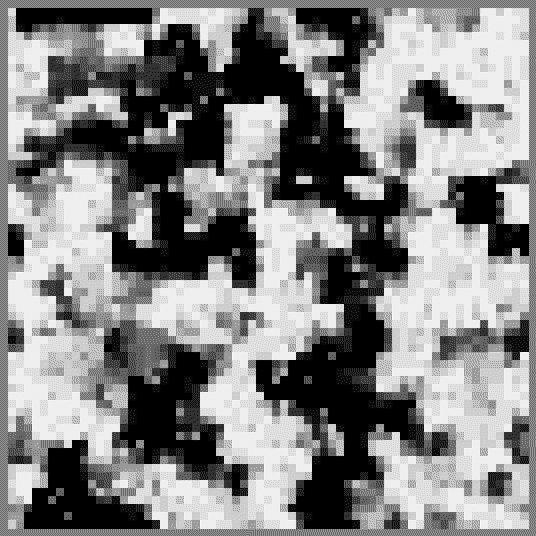
\includegraphics{array_snapshot_square.jpg}} &
\scalebox{0.27}{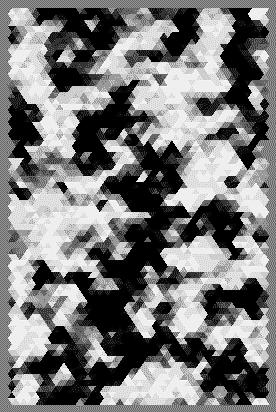
\includegraphics{array_snapshot_trig.jpg}} &
\scalebox{0.27}{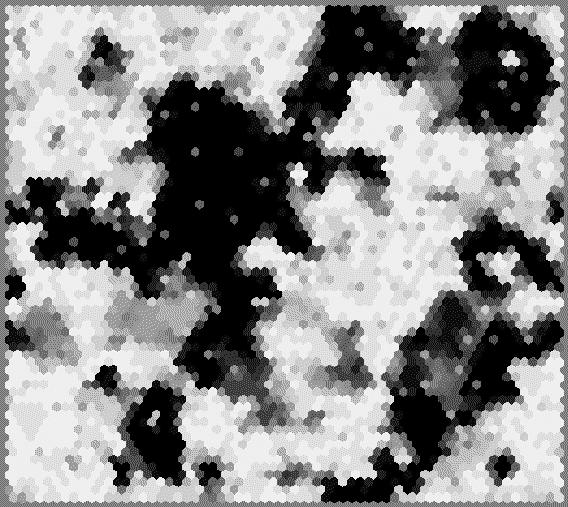
\includegraphics{array_snapshot_hex.jpg}}\\
(a) & (b) & (c)
\end{tabular}
\caption{The complex arrays in \stochsim{} 1.4 can have geometries
  based on (a) squares, (b) triangles or (c) hexagons.  Images such as
  these can be generated from the snapshot output of \stochsim{} by
  using the script \texttt{arraydraw.py} to generate images such as
  these.}
\end{center}
\label{fig-geometry}
\end{figure}

\section{Setting up a simulation that uses 2-D complex arrays
  (\texttt{STCHSTC.INI})}

In order to tell the \stochsim{} program that 2-D complex arrays will be
used in a simulation, the following optional parameters must be
specified in the main simulation configuration file (\texttt{STCHSTC.INI}).

\subsection{[Options]}
\begin{description}
\item[UseSpatialExtensions] This parameter specifies whether or not
  \stochsim{}'s spatial extensions will be used in a simulation.  This
  value must be set to 1 when using 2-D complex arrays. When this is
  set to 0, \stochsim{} ignores the following two parameters and behaves
  exactly like \stochsim{} 1.0.
\end{description}

\subsection{[File Names]}
\begin{description}
\item[ArrayINIFile] The path name specifying the location of the
  complex array configuration file (e.g. ``\texttt{./ARRAY.INI}'').
  
\item[ArrayOutPrefix] A path name which will be the prefix of all
  array output files (e.g. ``\texttt{../Output/}'').  The final name
  of each complex array output file (e.g. \\
  ``\texttt{../Output/ARRAY\_SNAPS\emph{X}.OUT}'') will consist of a suffix
  appended to this prefix.
\end{description}



\section{Definition of complex arrays (\texttt{ARRAY.INI})}\label{array_ini}

The complex array configuration file can take any name, as long as it
matches the name specified in the simulation configuration file, but
we recommend using something fairly obvious (e.g.
``\texttt{ARRAY.INI}'').  This file consists of three or more
sections: one \textbf{[General]} section, one \textbf{[Neighbour
  Sensitive Complex Types]} section\footnote{As of version 1.4, the
  preferred location of this section is in the complex configuration
  file (\texttt{COMPLEX.INI}).}, one or more
\textbf{[\emph{ARRAY\_NAME}]} (where \emph{ARRAY\_NAME} is the name of
the array) sections, and zero or more \textbf{[Snapshot Variable
  \emph{X}]} (where \emph{X} is a number) sections.  An
\textbf{[\emph{ARRAY\_NAME}]} section must be defined for each complex
array to be used in the model, and a \textbf{[Snapshot Variable
  \emph{X}]} section must be defined for each snapshot output that is
desired (see section \ref{se_output}). The parameters which must be
specified in each section are as follows:

\subsection{[General]}
\begin{description}
\item[Arrays] The list of complex arrays to be used.  The name of each
  array must be given here as a comma-separated list.
  
\item[DumpInterval] The interval between times at which complex array
  dumps should be stored (floating point).

\item[NumSnapshotVariables] The number of snapshot variables that are
  defined in this file (integer).
\end{description}

\subsection{[Neighbour Sensitive Complex Types]}
Note that as of version 1.4, the preferred location of this section is
in the complex configuration file (\texttt{COMPLEX.INI}).  If it is
defined in both files, the definition in the complex array
configuration file (\texttt{ARRAY.INI}) will be ignored.

\begin{description}
\item[NeighbourSensitiveComplexes] A comma-separated list of symbols,
  one for each neighbour-sensitive complex type in the reaction
  system.
  
\item[\emph{S}\_NS\_INIFile] For each NS-Complex type in the model, a
  line of the following form must be specified here:\\[\baselineskip]
  \emph{S}\_NS\_INIFile = \emph{Path}\\[\baselineskip]
  where \emph{Path} is the path name of the configuration file for the
  NS-Complex type \emph{S} (usually named \texttt{NS\_\emph{X}.INI},
  where \emph{X} is a number).
\end{description}

\subsection{[\emph{ARRAY\_NAME}]}
\begin{description}
\item[Complex] The name of the complex type that constitutes this
  complex array.
  
\item[NeighbourSensitive] Whether the complex type that constitutes
  this complex array is neighbour sensitive (must always be set to 1
  in present implementation).

\item[Geometry] The geometry of the complex array (must be one of
  ``Square'', ``Triangle'' or ``Hexagon'').

\item[BoundaryCondition] The boundary condition to be used for this
  complex array (0 = Toroidal, 1 = Real boundaries).

\item[XDimension] The length of the X-axis of the complex array (integer).

\item[YDimension] The length of the Y-axis of the complex array (integer).
  
\item[CreateDumpFile] Whether or not the state of this complex array
  should be dumped to a file during simulation (1 = Yes, 0 = No).
  Note that array dumps are different from array snapshots!
  
\item[EquilibrationInterval] The interval between times at which this
  complex array is to be equilibrated (floating point).  All rapid
  equilibria defined for each complex within the complex array will be
  equilibrated at this frequency.
\end{description}

\subsection{[Snapshot Variable \emph{X}]}
\begin{description}
\item[Array] The name of the array that this snapshot variable represents.
\item[States] A comma-separated list of bit strings (or wildcard
  strings) that represent all the states that this snapshot variable
  will represent.  It is convenient to use wildcard strings here, if
  you want to monitor the state of specific flags (e.g.  ``1?0?'', for
  a complex with four state flags when you want to highlight all
  complexes with the first flag on and the third flag off).
  
\item[StoreInterval] The interval between the times at which values
  of this snapshot variable are to be stored (floating point).

\item[AveragedOutput] Specifies whether snapshot output of array
  states should be be instantaneous or time-lapse (0 = instantaneous,
  1 = time-lapse).
  
\item[AverageInterval] If time-lapse snapshots are desired, give the
  length of the interval to use for averaging (floating point; must be
  smaller than value specified for \textbf{StoreInterval}).  This
  parameter is ignored if \textbf{AveragedOutput} is set to 0.
  
\item[SampleInterval] If time-lapse snapshots are desired, give the
  interval between times at which values should be sampled for
  averaging (floating point; must be smaller than value specified for
  \textbf{AverageInterval}).  This parameter is ignored if
  \textbf{AveragedOutput} is set to 0.
\end{description}

\section{Definition of neighbour-sensitive complexes (\texttt{NS\_\emph{X}.INI})}
\subsection{[General]}
\begin{description}
\item[NumRapidEqm] The number of state flags of this NS-Complex that
  are controlled by NS-RapidEqm's (integer).  Note that this number
  should only include the number of NS-RapidEqm's, and not normal
  RapidEqm's, which are be defined separately in the multistate
  complex configuration file (\texttt{MS\_\emph{X}.INI}).
  
\item[Reactions] A comma-separated list of reaction identifiers for
  NS-Reactions.  Be careful to use the same identifiers as specified
  in the reaction configuration file (\texttt{REACTION.INI}) and multistate
  configuration file.
  
\item[NumNeighbours] The number of nearest neighbours that this
  NS-Complex has in the complex array (integer). Note that
  this number must correctly match the geometry of the complex array
  that this NS-Complex will be inserted into (3 for ``Triangle'', 4
  for ``Square'' and 6 for ``Hexagon'').  
\end{description}

\subsection{[Rapid Equilibrium \emph{X}]}
Each NS-RapidEqm must have a section headed [Rapid Equilibrium
\emph{X}] where \emph{X} is the number of the rapid eqm
\begin{description}
\item[Flag] The name of the state flag which is controlled by an
NS-RapidEqm. ``State'' is also accepted for backward compatibility but
  is deprecated.
  
\item[CoupledStates] A comma separated list of wildcard strings (do
not use whitespaces), representing the states of nearest neighbours
that are coupled to this NS-RapidEqm.

\item[Wildcards] A comma-separated list of all bit strings below which
  contain one or more of the wildcard character, '?'. Wildcards
  represent \emph{both} 0 and 1.
  
\item[\emph{BitString}] Defines the NS-RapidEqm probabilities
  associated to specific states.  The parameter name,
  \emph{BitString}, can be a bit string representing a single state,
  or a wildcard string representing multiple states.  If wildcard
  strings are used, they must also be declared in the
  \textbf{Wildcards} parameter described above.  The probabilities
  defined in each line are applied only when the complex is in a state
  which matches that (those) specified in the parameter name.  The
  value of this parameter must be a comma separated list of
  rapid-equilibrium probabilities.  The number of probabilities in
  this list must be exactly \textbf{NumNeighbours} + 1. These
  correspond to the rapid-equilibrium probabilities of the flag
  (specified by the \textbf{Flag} parameter in this section) when
  zero to \textbf{NumNeighbours} neighbours are in a coupled state.
  Multiple instances of this line should be defined, if necessary.
  For states that are not defined here, a default probability of zero
  is assigned automatically.
\end{description}

\subsection{[Reaction \emph{XD}]}
Each reaction involving a NS-Complex must have a section [Reaction
\emph{XD}] where X is the reaction number and D is direction ('F' or
'R').
\begin{description}
\item[ReactNeighbourID] A numerical identifier specifying the reacting
  neighbour (e.g. for the ``Square'' geometry, 0 = North, 1 = East, 2
  = South, 3 = West).

\item[EffectOnNeighbour] A comma-separated list of state changes on
the reacting neighbour resulting from this reaction.  A '+' character
before the name of the affected flag indicates that the flag is set (0
-> 1); a '-' character indicates that the flag is cleared (1 -> 0);

\item[Wildcards] A comma-separated list of all bit strings below which
  contain one or more of the wildcard character, '?'. Wildcards
  represent \emph{both} 0 and 1.

\item[\emph{BitString}] Defines the NS-Reaction relative rate
(floating point; 0 <= \emph{p} <= 1) associated to specific states.
The parameter name, \emph{BitString}, can be a bit string representing
a single state, or a wildcard string representing multiple states.
The probability defined in each line are applied only when the complex
is in a state which matches that (those) specified in the parameter
name.  Multiple instances of this line should be defined, if
necessary. For states that are not defined here, a default probability
of zero is assigned automatically.
\end{description}

\section{Output of complex-array states}\label{se_output} 

\subsection{A note for StochSim 1.2 users}
Before reading this section, please note that the way in which the
output of complex-array states are specified in the INI files has
undergone considerable changes between \stochsim{} 1.2 and 1.4.  In
this section we will only describe the new way of specifying the
output which only applies to \stochsim{} 1.4 and later.  If you are
still using \stochsim{} 1.2, we recommend that you upgrade to
\stochsim{} 1.4, which incorporates various new features and also has
been further optimised for speed.  However, if for some reason you
wish to keep using \stochsim{} 1.2, please refer to the older versions
of this manual.

\subsection{Array snapshots}
\stochsim{} 1.2 and later versions can output the state of an entire
complex array at any given time during simulation as graphical
representations called \emph{snapshots}.  In a snapshot, each
NS-Complex in the complex array is represented by a polygon
(corresponding to that specified for the array geometry\footnote{Note
  that in \stochsim{} 1.2, only the ``Square'' geometry was
  supported.}), so the entire image representing the array will be a
tesselation of polygons.  You can specify a single state
or a combination of states of the NS-Complex that you want highlighted
in the snapshot, so that the spatial distribution of specific states
that you are interested in can be visualised.

There are two types of snapshots that can be created,
\emph{instantaneous} and \emph{time-lapse} (see Figure
\ref{fig-snapshots}).  Instantaneous snapshots are snapshots in which
the instantaneous state of the complex array is recorded (i.e. the
value of each pixel is either 0 or 1).  Time-lapse snapshots are
snapshots in which the value of every pixel in the snapshot is
averaged over time (i.e. the value of each pixel is between 0 and 1).

\begin{figure}
\begin{center}
\resizebox{3.5cm}{3.5cm}{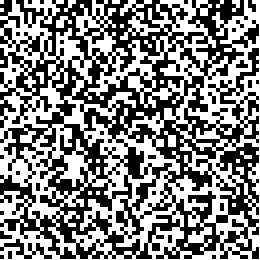
\includegraphics{array_snapshot_inst.jpg}}
\hspace{1cm}
\resizebox{3.5cm}{3.5cm}{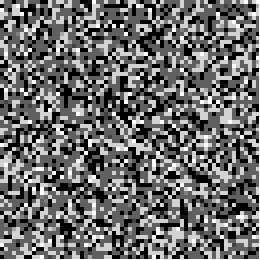
\includegraphics{array_snapshot_ave.jpg}}\\
(a) \hspace{4cm} (b)
\end{center}
\caption{\stochsim{} 1.2 and later versions can output
  (a) instantaneous snapshots, or (b) time-lapse snapshots of an array
  of NS-Complexes.  The tiled polygons of an instantaneous snapshot
  are either white or black.  The polygons of a time-lapse snapshot
  have grey level somewhere between white and black, depending on the
  proportion of time that the corresponding NS-Complex spent in the
  highlighted state.}
\label{fig-snapshots}
\end{figure}

In the instantaneous snapshots, white pixels represent NS-Complexes
which are in the highlighted state, and black pixels represent
NS-Complexes in all other states.  In the time-lapse snapshots, grey
levels are assigned to the pixels according to the proportion of time
each NS-Complex object has spent in the highlighted state (i.e.
NS-Complexes which were in the highlighted state 100\% of the time
will show up white, and NS-Complexes which were never in the
highlighted state will show up black).

Snapshots are recorded at a user-specified frequency during the
simulation.  Time series of snapshots are recorded in output files
named \texttt{ARRAY\_SNAPS\emph{X}.OUT}, where \texttt{\emph{X}} is a
numerical identifier for each series of snapshots.  Each file contains
snapshots with different highlighted states.  Each of these snapshot
files is essentially a concatenated series of X Pixmap (XPM) format
image files.  To view each snapshot, the snapshot file must be split
into separate image files.  As of version 1.4, a novel utility program
called \texttt{arrayview.py} for this purpose is providedin the
\texttt{bin} directory of the \stochsim{} distribution.  This program
can generate a series of GIF files from a StochSim snapshot file.  It
will also automatically determine the geometry of the array from the
snapshot file, and draw triangles, squares or hexagons as necessary
(see Figure \ref{fig-geometry}).  \texttt{arraydraw.py} is written in
Python, which works on just about all modern operating systems, and
comes installed as standard on most UNIX operatins systems these days.
To run \texttt{arrayview.py}, simply type
\\[\baselineskip]
\texttt{ \% arraydraw.py \emph{snapshot\_file} [edge\_length] }
\\[\baselineskip]
at the UNIX command-line. \texttt{[edge-length]} is an optional
argument which tells \texttt{arraydraw.py} how long you want the edges
of the polygon to be.  If you are using Microsoft Windows or a UNIX
operating system without python installed, you must first download and
install the python interpreter (available from
\url{http://www.python.org}).  Once the images have been generaged,
any image viewer can be used to view the images.

If you want to created animations from the image files, you can use
external programs such as \texttt{gifsicle} (available from
\url{http://www.lcdf.org/gifsicle/}), which can generate GIF
animations from a series of GIF image files.

\subsubsection{Example: How to set up the output of snapshots}
Let's say you have an array of receptors named ``ARRAY1''. The
NS-Complex which makes up this array has two state flags.  The first
flag, named ``L'', represents the state of the ligand binding site (1
= bound; 0 = unbound). The second flag, named ``X'', represents the
conformational state of the receptor (1 = active conformation; 0 =
inactive conformation).  Now, let us suppose that you want to monitor
both the changes in activity and ligand binding of all the receptors
in the array, averaged over time.  For this you will need two series
of time-lapse snapshots, one to monitor the activity, and one to
monitor the state of the ligand binding site.

To specify the snapshots you want, you must set up a \textbf{Snapshopt
  Variable} for each snapshot.  These are defined in the complex array
configuration file (\texttt{ARRAY.INI}).  Each snapshot variable must
be defined in its own \textbf{[Snapshot Variable \emph{X}]} section,
which has seven parameters (see section \ref{array_ini} for formatting
details).  The first five parameters must be defined for all snapshots
.  The first parameter, \textbf{Array} specifies the name of the array
that the snapshot variable will represent.  The next parameter,
\textbf{State} specifies the states of the NS-Complex that this
variable will highlight in the snapshot output, using a
  comma-separated list of bit strings (or wildcard strings).
\textbf{StoreInterval} specifies how often snapshots from this
variable are to be output during the simulation, and
\textbf{AveragedOutput} is a boolean parameter specifying whether or
not the output snapshots should be averaged over time (set to 1 if
averaging is desired, and 0 otherwise).  If \textbf{AveragedOutput} is
set to 1, the parameters \textbf{AverageInterval} and
\textbf{SampleInterval} must also be set.  \textbf{AverageInterval} is
the length of the interval over which the snapshot values will be
averaged, and \textbf{SampleInterval} is the inverval between times at
which values are sampled for averaging.  For this example, we will use
0.1 for the store and average intervals, and 0.001 for the sample
interval.  Note that the value of \textbf{AverageInterval} cannot be
larger than \textbf{StoreInterval}, and \textbf{SampleInterval} cannot
be larger than \textbf{AverageInterval}.

% When specifying \textbf{StoreInterval} and
% \textbf{AverageInterval}, the characteristic rates of whatever
% processes control the state changes being monitored should be
% considered (e.g. if the rate of a reaction controlling a certain flag
% is about 10 s\textsuperscript{-1}, you should set StoreInterval to
% smaller than 0.05).

So, for the example here, you would define two Snapshot Variables.
The two sections defining these variables would like this:
\begin{small}
\begin{verbatim}
[Snapshot Variable 1]    ;; Snapshot variables must be numbered sequentially
Array           = ARRAY1 ;; Specify the name of the array here
States          = 1?     ;; States matching this wildcard string are hi-lited
Name            = RL     ;; You can name variables as you like
StoreInterval   = 0.1    ;; Interval between storage times (s)
AveragedOutput  = 1      ;; Indicates whether output should be averaged
AverageInterval = 0.1    ;; Length of averaging interval (s)
SampleInterval  = 0.001  ;; How often values are sampled for averaging (s)

[Snapshot Variable 2]    
Array           = ARRAY1 
States          = ?1     
Name            = RX     
StoreInterval   = 0.1    
AveragedOutput  = 1      
AverageInterval = 0.1    
SampleInterval  = 0.001  
\end{verbatim}
\end{small}

The wildcard strings specified for the \textbf{State} parameters,
``1?'' (matches both ``10'' and ``11'') tells \stochsim{} to create a
series of snapshots that highlight NS-Complexes with the first flag on
(receptors with ligand bound), and ``?1'' (matches both ``01'' and
``11'') tells \stochsim{} to create another series of snapshots that
highlight NS-Complexes with the second flag on (active receptors).

That's it!  You should find two new output files after the
simulation, one named \texttt{ARRAY\_SNAPS1.OUT} (with the
ligand-bound receptors highlighted) and another named
\texttt{ARRAY\_SNAPS2.OUT} (with the active receptors highlighted).

\subsection{Array dumps}
As of version 1.4, \stochsim{} can output the complete state of the
complex array in ``dump files'' which can later be used to resume the
simulation from the time at which the state was dumped.  If such an
output is desired for an array, the parameter \textbf{CreateDumpFile}
in the \textbf{[\emph{ARRAY\_NAME}]} section must be set to 1.  The
frequency at which all array dumps will be output to dump files must
be specified using the parameter \textbf{DumpInterval} in the
\textbf{[General]} section of the complex array configuration file
(\texttt{ARRAY.INI}).

%\section{Manipulating the array output}
%       *monochrome
%       *colour

%%% Local Variables: 
%%% mode: latex
%%% TeX-master: "stochsim_manual"
%%% End: 

\chapter{Tk\stochsim{}: user guide}

The original \stochsim{} simulator was written for Microsoft Windows and was
provided with a graphical user interface (GUI) based on the Microsoft MFC
widgets.  Although the core simulation engine was written an ANSI C++, and
therefore could be ported to other operating systems with relative ease, the
widgets used for the GUI were not compatible with other operating systems such
as UNIX, Linux, or MacOS.  Therefore to run \stochsim{} under such operating
systems, the user was required to write the simulation initialisation files
manually. This is tedious and error-prone. In order to ease the creation and
modification of simulation configurations under a larger number of operating
environments, a novel interface written in Perl using the Tk widgets was
developed. This interface has been written and tested under Debian/GNU Linux,
but should run under most modern operating systems for which a Perl/Tk exists
(It has also been tested under Microsoft Windows98). The current interface
requires at least Perl 5.005 and Perl/Tk 800.022. 

\parpic[r]{\scalebox{0.4}{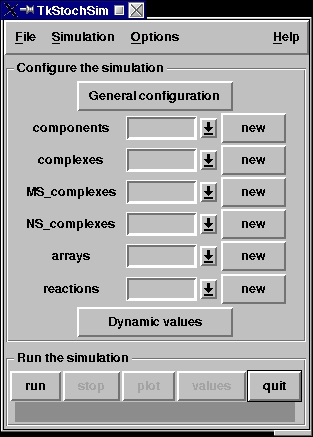
\includegraphics{main.jpg}}} When Tk\stochsim{} is
launched, the main window appears on the screen.  Tk\stochsim{} can be
controlled with either the mouse or the keyboard.  When using the keyboard,
pressing the <tab> key allows you to switch the focus between the various
widgets (buttons, text boxes, etc.) of the interface.  A focused widget can be
activated by pressing the <space> bar or the <return> key. The menus can also be
activated via the keyboard by the sequences \mbox{<Alt-f>} (``File'' menu),
\mbox{<Alt-s>} (``Simulation'' menu), \mbox{<Alt-o>} (``Option'' menu) and
\mbox{<Alt-h>} (``Help'' menu). You can quit the program by clicking on the
``quit'' button or pressing \mbox{<Ctrl-q>}.

The ``File'' menu is used to open an existing simulation (accelerator:
\mbox{<Ctrl-o>}), to save the current configuration (accelerator:
\mbox{<Ctrl-s>}), to create a new simulation or to rename the current simulation
(accelerator: \mbox{<Ctrl-a>}) or to quit (accelerator: \mbox{<Ctrl-q>}). You
can also import or export simple simulations using the SBML language
level1\footnote{See
  \url{http://www.cds.caltech.edu/erato/sbml/docs/index.html}.}  designed by the
\textsc{erato} project on systems biology.  The ``File'' menu also presents a
history of past simulations, providing an easy and fast access to them.
  
The ``Simulation'' menu currently presents only two options, one to run a
simulation (accelerator: \mbox{<Ctrl-r>}) and one to stop the simulation
(accelerator: \mbox{<Ctrl-w>}). This last option is currently not activated
under Microsoft Windows.

The ``Options'' menu permits to configure the interface and to activate or
deactivate the helping balloons on the fly (accelerators: \mbox{<Ctrl-b>} and
\mbox{<Ctrl-n>} respectively).  Those balloons present a short explanation on
the use of the different items of the interface. It is a good idea to explore
the graphical interface at least once with the balloons activated. You can
systematically desactivate the balloons by setting the ``balloon'' option to off
in the file \texttt{stochsimrc}.  This file is present in the directory ``lib''
of the distribution. It contains information about the setup of the Perl/Tk
interface.  A copy of this file is normally installed in the personal directory
\texttt{.stochsim} of each user (or in the directory \texttt{config\_examples}
under Microsoft Windows9x). The configuration of the interface can be partially
done through the \emph{Preferences} window (accelerator: \mbox{<Ctrl-P>}).  All
the changes will be recorded in \texttt{stochsimrc} when the program will quit.
The file can also be manually edited with any text editor.

Finally, the ``help'' menu provides the legal informations about the programs
and access to a PDF version of the present manual. The
first time you'll ask for the PDF version, the program shall ask you to point
the location of your favourite PDF reader. It will normally remind it afterward.
The address is kept by the option ``pdfreader'' in the file \texttt{stochsimrc}.

All the accelerators described should be directly available from the main
window, without the need to open the menus.

\section{Opening and saving a simulation}

All the simulations should normally be stored in a specific directory (although
this is not an obligation). Under Unix-like systems, this
directory is \texttt{\$HOME/.stochsim}. Under Microsoft Windows9x the
simulations are stored in the subdirectory \texttt{config\_examples} of the
\stochsim{} distribution.  Each simulation is stored in a subdirectory, the
name of which is specified by the user. The structure of this directory is
constant.  It contains two subdirectories, \texttt{Input} and \texttt{Output},
containing the \texttt{*.INI} and \texttt{*.OUT} files respectively.

To open an existing simulation, you can go to the menu-bar and select
``File->Open...'', or type \mbox{<Ctrl-o>}. Then select an existing simulation
configuration file (usually named \texttt{STCHSTC.INI}). The usage of the file
selector could be lightly different according to the running operating system.
However, since it is the usual file selector of your windows manager, its
description is out of the scope of the present manual. Tk\stochsim{} will
remind the last directory visited to look for a simulation. It is stored by the
option ``confdir'' in the file \texttt{stochsimrc}. You can also setup the
default directory with the \emph{Preferences} window.

To save a configuration under its previous name, you can go to the menu-bar and
select ``File->Save'' or type \mbox{<Ctrl-s>}. Note that the current configuration
is automatically saved when a simulation is launched.

To create a new configuration or to save the current configuration under a
different name, you can to the menu-bar and select ``File->Save as...'' or type
\mbox{<Ctrl-a>}, and then select an existing \texttt{STCHSTC.INI} (in the
subdirectory \texttt{Input} of an existing simulation) or type the name of the
new \emph{main} directory.


\section{Setting up a simulation}

\subsection{General configuration}\label{genconfig}

\parpic{\scalebox{0.4}{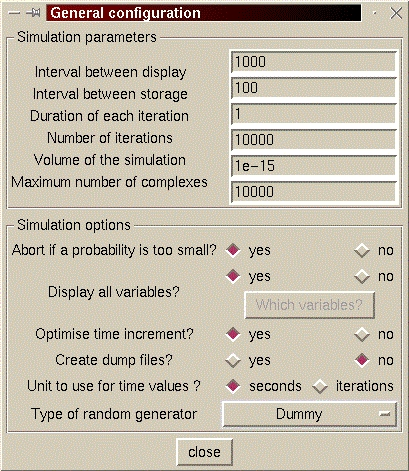
\includegraphics{mainconf.jpg}}} To create a new
simulation, you need to setup a general configuration first. To do so, click on
the button labelled ``General configuration''.  
% previous has to be located before the screenshot, but put here for easthetics
The \emph{General configuration} window is then opened, where you can modify
several options of the simulation.  The detailled explanation of the various
options is given in the chapter \ref{conf_files}. 

The ``interval between storage'' controls the frequency of the variable
recording, and hence the data shown in the graphical display (see section
\ref{display}). There is a relationship between the ``duration of the
simulation'' and the ``interval between storage''. You could be ask to change
the latter by \stochsim.

The option ``duration of each iteration'' is meaningfull only if you do not
allow the optimisation of the time increment. In such a case, you will have to
set-up the time increment by trial error. Indeed, if the time increment is too
small, the probability that no reaction takes place during an iteration becomes
significant and the simulation is inefficient. On the contrary, if the time
increment is too big, several reactions should take place during one iteration,
which cannot be the case with \stochsim{}. 

The limit for the ``maximal number of complexes'' is \MAXLIMITCOMPLEXES. This
value is far higher than what we can expect to use in a \stochsim{} simulation
anyway (except if you are ready to wait the results for twenty years). Be sure
to check the option ``use spatial extensions'' if you want to use the
bidimensional lattices implemented since \stochsim{} 1.2.

You'd rather not touch most of the options in the frame ``Simulation options''.
Their default value is fine for all simulations. However do not forget to
select ``Use spatial extensions'' if you want to setup an array of
neighbour-sensitive complexes (see section \ref{neighboursensitive}). 

If you choose to display only some selected variables, answer ``no'' to the
question ``Display all variables'' and click on the button labelled ``Which
variables''.  Be careful, you need to setup the complexes to be used in the
simulation before playing with the variables to display (see sections
\ref{make_complexes} and \ref{make_multistates}). It is advisable to setup the
output only when the simulation is entirely written.

\parpic{\scalebox{0.4}{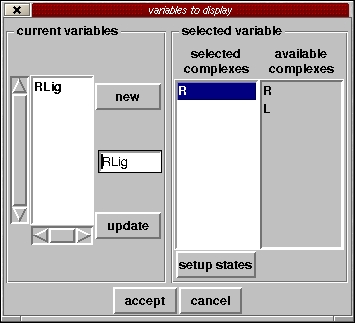
\includegraphics{vardispl.jpg}}} A new window, entitled
\emph{variables to display}, appears, presenting the current variables to
display. You can create a new variable or select existing ones. The maximal
number of variables you can display is \MAXNUMDISPLAYVARIABLES. To delete a
variable, select it and click while pressing the <Ctrl> key. Once a variable is
chosen, its name appears in the upper entry widget where you can change it.
The name of a variable to display is limited to \MAXOUTPUTVARNAMELENGTH{} characters.
As for several other entry widgets throughout the interface, the changes
of the name are recorded when the mouse quit the widget area, when you press
<Return> (\emph{not} the numeric pad <Enter>) or when another widget is focussed
(for instance with a <tab> press). The composition of the variable appears in
the middle-list. A variable can represent several complexes. You can add
complexes to the selected variable by drag and dropping them from the right
list. A variable can contain up to \MAXTYPESINOUTPUTVAR{} complexes. To delete a
complex from a variable, select it and click while pressing the <Ctrl> key. A
variable can represent specific states of a multistate complex. In such a case,
the variable can include only one complex type. To configure the states to be
displayed, select the complex and click on the button ``setup states''. If you
add another complex to a variable already containing a multistate complex, this
multistate is then considered as a regular complex and the variable is supposed
to display all its states. Therefore you cannot configure the states anymore.
This possibility reappears if you delete all the other complexes but the
multistate from the variable.

\parpic{\scalebox{0.4}{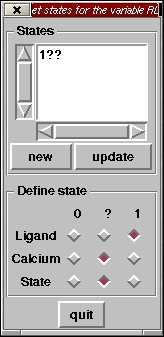
\includegraphics{displstates.jpg}}} When you decide to
choose which states of a multistate complex you want to
display\footnote{Remember, this is possible only if the variable contains only
  this multistate.}, a new window pops-up, entitled \emph{variable NAME}. A state
is defined by a certain configuration of all the flags (`set' or `1', `unset'
or `0' and `undefined' or `?').  You can create a new state with the ``new''
button (all the flags are initially at `?').  The various flags of the
multistate complex can be configured with the radiobuttons. As usual, after
having selected a state, you can click while pressing the <Ctrl> key to delete
it.

Once all your variables are set, you can record the changes you made and close
the \emph{variables to display} window by clicking the ``accept'' button. The
``cancel'' button will close the window without changing your configuration.

When you close the \emph{General configuration} window, the changes are
recorded. Be careful to undo all the changes you made if you want to ignore
them. Indeed there is currently no ``cancel'' button.

\subsection{Creating elementary components of the simulation}

The elementary building blocks of the simulation are the components, which
permit to make up the complexes, i.e. the actually reacting entities.  You can
select an existing component with the browsing list, or click on the nearby
``new'' button to create a new one. Up to \MAXCOMPONENTS{} components can be
created per simulation.

\parpic{\scalebox{0.4}{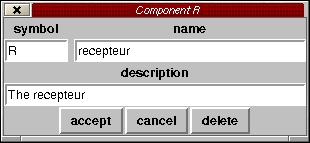
\includegraphics{component.jpg}}} A \emph{Component
  [SYMBOL]} window pops-up, allowing the configuration of the component
\emph{SYMBOL}.  In this window, you can enter a symbol for the component, a
name, and a description. The symbol is important since it will be used to
construct the name of the complexes including this component (maximal length
\MAXCOMPONENTSYMBOLLENGTH{} characters). Note that symbols can overlap but
cannot be included one into another. For instance, symbols AB and AC can
coexists, but not symbols A and AB. This insure the unequivocal decomposition of
the symbol of a complex into its components (see section \ref{make_complexes}).
The name can be longer and more explicit (maximal length
\MAXCOMPONENTNAMELENGTH{} characters). For instance the symbol can be `p' and
the name ``phosphate''.

Clicking the three lowest buttons will close the \emph{Component [SYMBOL]}
window, either recording the changes, cancelling them or totally removing the
component. A component cannot be removed if it is part of a complex.

\subsection{Creating complexes involved in the simulation}\label{make_complexes}

The complexes are the actual reacting entities of the simulation. You can select
an existing complex with the browsing list, or click on the nearby ``new''
button to create a new one. Up to \MAXCOMPLEXTYPES{} different complexes can be
created per simulation.

\parpic{\scalebox{0.5}{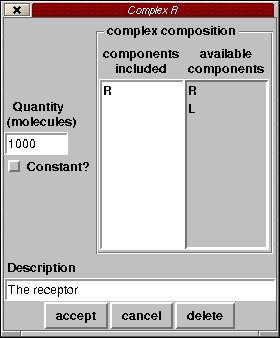
\includegraphics{complex.jpg}}} A \emph{Complex [SYMBOL]}
window pops-up, allowing the configuration of the complex \emph{SYMBOL}. To add
a component to the current complex, drag it from the rightmost list to the left
one. To remove a component from the current complex, select it from the leftmost
list and click while pressing the <Ctrl> key. \emph{The order of the components
  is important. A complex made of A then B is different from a complex made of B
  then A}. This allows the definition of complexes which include several times
the same component, but in different places or the definition of complexes made
up of the same components in different order. Up to \MAXCOMPONENTSINCOMPLEX{}
components can be part of a complex.  In the left entry widget, enter the
initial quantity of this complex, at the beginning of the simulation.  Note that
this must be expressed in number of molecules, not in concentration. If you
check the tickbox ``Constant?'', the concentration of that complex will be
maintained constant throughout the simulation\footnote{In order to do that, the
  GUI tranforms all the bimolecular reactions into unimolecular reactions,
  merging the rate constants and the concentrations of the constant substrates.
  In the Lotka-Voltera example provided with the distribution, compare for
  instance the values of the kf rate constant for the reaction
  $X+Y_1\rightarrow2Y_1$ shown in the GUI and in the file
  \texttt{REACTION.INI}.}. Be careful not to fix the concentration of a complex
involved in unimolecular reactions, or to fix the concentration of a multistate
complex.

Clicking the three lowest buttons will close the \emph{Complex [SYMBOL]}
window, either recording the changes, cancelling them or totally removing the
complex. A complex cannot be removed if it is part of a reaction or if a
multistate complex is based on it.

\newpage

\subsection{Creating multistate complexes}\label{make_multistates}

The multistate complexes are a special kind of reacting entities which possess
several binary flags describing their various possible states (see section
\ref{intro_multistates}).  You can select an existing multistate complex with
the browsing list, or click on the nearby ``new'' button to create a new one.

\parpic{\scalebox{0.5}{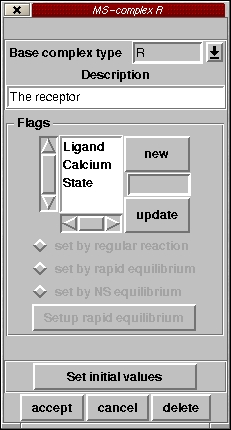
\includegraphics{multistate.jpg}}} A \emph{MS-complex
  [SYMBOL]} window pops-up, allowing the configuration of the multistate complex
\emph{SYMBOL}.  Each multistate complex has to be based on one of the complexes
previously defined (see section \ref{make_complexes}). If a complex is already
defined as multistate, you cannot use it for another multistate configuration
(create another complex instead). You can change the complex a multistate is
based on. If you do that \emph{the previous multistate configuration will be
  deleted}. This feature cannot currently be used to duplicate multistate
configuration between complexes.

You can create new flags (``new'' button). The name of a flag cannot have more than
\MAXMSFLAGLENGTH{} characters. To remove a flag from the complex, select it
and click while pressing the <Ctrl> key. Up to \MAXMSNUMFLAGS{} can be created
for each multistatee  complex.

The state of each flag can be controlled either by a standard reaction (see
section \ref{reactions}), or by a rapid equilibrium (see section \ref{ms_ini})
(if you are using the spatial extensions, there are actually two different kinds
of rapid equilibria, see section \ref{neighboursensitive}). You can change the
mode of control of each flag.  However, be careful and take a break before to do
so. Indeed, a quite complex configuration of a rapid equilibrium can be easily
wiped-out if you decide to reverse to a control by a ``regular'' reaction. In
order to change the control mode from ``reactions'' to ``rapid equilibrium'',
all the reactions involved have to be suppressed before.

If a flag has to be controlled by a classical multistate rapid equilibrium, you
have to setup the probability that it is ON, depending on the state of the
entire complex. To do so, press on the button ``Setup rapid equilibrium''.

\parpic{\scalebox{0.5}{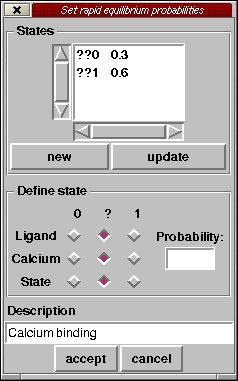
\includegraphics{MSrap_equil.jpg}}} A window \emph{set
  rapid equilibria properties} pops-up. You can create new states with the
``new'' button, and specifies the configuration of each flag with the
radiobuttons.  After selecting a state, you can click while pressing the <Ctrl>
key to delete it. The probability to set the controlled flag, depending on the
state of all the other flags, can be entered in the right entry widget.If you
add a flag later on, its value will be set at `?' in all the rapid-equilibria
and reaction states\footnote{This is also true for all the variables to display
  and the array snapshots by the way.}.

A rapid equilibrium can be controlled by a dynamic value (see section
\ref{dynamic_ini}). In such a case, the value you enter here has to be the
highest probability for the flag to set. This value will be replaced by the
adequat dynamic value when the event timepoints will arrive.

Once your probabilities are set, you can record the changes you made and close
the \emph{rapid equilibrium} window by clicking the ``accept'' button. The
``cancel'' button will close the window without changing your configuration.

Once all the flags are defined, the initial quantity of the complex in the
various states at the beginning of the simulation can be setup.

\parpic{\scalebox{0.5}{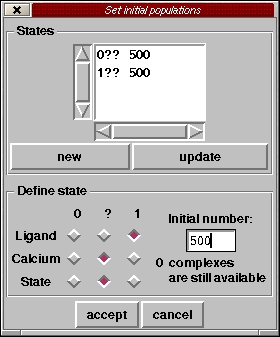
\includegraphics{ms_states.jpg}}} A click on the button
``Set initial values'' will cause a new window to pops-up, entitled \emph{Set
  initial populations}.  Several states can be defined by setting up the various
flags of the multistate complex. You can create new states with the ``new''
button.  For each particular state, you can specify the number of complexes in
this state at the beginning of the simulation. The sum of all states cannot be
superior to the total initial number of the current complex, defined previously
(see \ref{make_complexes}).  As usual after selecting a state you can click
while pressing the <Ctrl> key to delete it.

Once all the desired initial values are set, you can commit the changes and
quit (``accept'' button) or quit without recording changes (``cancel'' button).

Clicking the three lowest buttons of the \emph{MS-complex [SYMBOL]} window will
close it, either recording the changes, cancelling them or totally removing the
multistate configuration of the complex. Note that a multistate configuration
cannot be suppressed if a neighbour-sensitive complex is based on that
multistate complex.

\subsection{Creating neighbour-sensitive complexes}\label{neighboursensitive}

The neighbour-sensitive complexes are a special kind of multistate complexes
which can react according to the state of their nearest neighbours. They will
form the elements of bidimentional lattice you will setup later on (see section
\ref{arrays}). You can select an existing neighbour-sensitive with the browsing
list, or click on the nearby ``new'' button to create a new one.

\parpic{\scalebox{0.5}{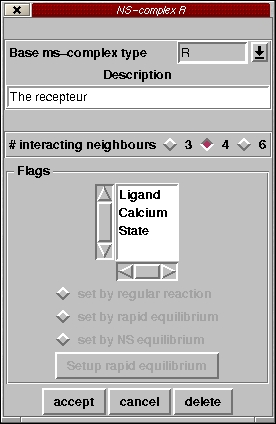
\includegraphics{neighboursensitive.jpg}}} A
\emph{NS-complex [SYMBOL]} window pops-up, allowing the configuration of the
neighbour-sensitive complex \emph{SYMBOL}.  Each neighbour-sensitive complex has
to be based on one of the multistate complexes previously defined (see section
\ref{make_multistates}). If a multistate complex is already defined as
neighbour-sensitive, you cannot use it for another neighbour-sensitive
configuration (create another complex instead). You can change the multistate
complex a neighbour-sensitive is based on. If you do that \emph{the previous
  neighbour-sensitive configuration will be deleted}. This feature cannot
currently be used to duplicate neighbour-sensitive configuration between
complexes.

The state of each flag can be controlled either by a standard reaction (see the
section \ref{reactions}), or by a rapid equilibrium (see section \ref{ms_ini}).
If you are using the spatial extensions, there are actually two different kinds
of rapid equilibria \footnote{You would not read that part if you aren't, or
  would you?}. You can change the mode of control of each flag.  However, be
careful and take a break before to do so. Indeed, a quite complex configuration
of a rapid equilibrium can be easily wiped-out if you decide to reverse to a
control by a ``regular'' reaction.  In order to change the control mode from
``reactions'' to ``NS rapid equilibrium'', all the reactions involved have to be
suppressed before.

If a flag has to be controled by a neighbour-sensitive rapid equilibrium press
on the button ``Setup rapid equilibrium''.

\parpic{\scalebox{0.5}{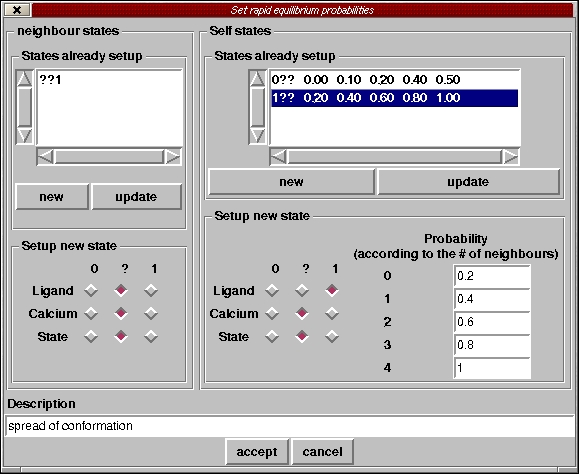
\includegraphics{NSrap_equil.jpg}}} A window \emph{set
  rapid equilibria properties} pops-up. You have to setup the probabilities that
it is ON, depending on the state of the entire complex (rightmost frame),
\emph{as well as the states of its nearest-neighbours} (leftmost frame). To do
so, If a complex has N neighbours (N depending on the geometry of the lattice
containing this neighbour-sensitive complex), N+1 probabilities have to be set
for each defined state, corresponding to 0,1 \ldots N neighbours being in the
particular states defined in the leftmost frame.

In both frames you can create new states with the ``new'' button, and specifies
the configuration of each flag with the radiobuttons. After selecting a state,
you can click while pressing the <Ctrl> key to delete it. The probabilities to
set the controled flag, depending on the state of the other flags, can be
entered in the right entry widgets.

Once your probabilities are set, you can record the changes you made and close
the \emph{rapid equilibrium} window by clicking the ``accept'' button. The
``cancel'' button will close the window without changing your configuration.

Clicking the three lowest buttons of the \emph{NS-complex [SYMBOL]} window will
close it, either recording the changes, cancelling them or totally removing the
neighbour-sensitive configuration of the complex.

\subsection{Configuration of the bidimensional lattice}\label{arrays}

In order to react with their neighbours, the neighbour-sensitive complexes have
to be arranged into bidimensional lattice, or arrays. A simulation can contain
several arrays. You can select an existing array with the browsing list, or
click on the nearby ``new'' button to create a new one. Up to 
\MAXNUMCOMPLEXARRAYS{} arrays can be created by simulation.

\parpic{\scalebox{0.5}{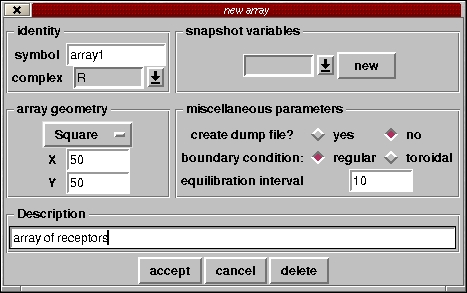
\includegraphics{array.jpg}}} A window \emph{Array
  [SYMBOL]} pops-up, allowing the configuration of the array \emph{SYMBOL}.  See
the section \ref{array_ini} for more details about the various options.  In the
frame ``Identity'', you can chose a symbol for the array (maximum
\MAXARRAYNAMELENGTH{} characters) and select the neighbour-sensitive complex it
will be made of.  The current version of \stochsim{} use only homogenous arrays,
made of one type of complex only.

The
frame ``Array geometry'' permits to setup the size of the array, but also its
topology, i.e. the number of neighbours each complex can react with. The maximal
allowed width is \MAXARRAYWIDTH{} and the maximal allowed length is
\MAXARRAYLENGTH{}.

If the ``boundary condition'' is set to ``regular'', a complex located on the
edge of the array will have less neighbours than the others. On the contrary,
if the the ``boundary condition'' is set to ``toroidal'', the opposite edges
are connected, giving the array the topologie of a doughnut. In this
configuration, all complexes have the same number of complexes.  The
``equilibration interval'' value controls the frequency of the re-equilibration
of all the flags controlled by a neighbour-sensitive rapid equilibrium.

The snapshot-variables are the spatial equivalent of the variable to display.
They represent selected states of each complex in the array. You can select an
existing snapshot-variables with the browsing list, or create a new one by
clicking on the nearby ``new'' button. Up to \MAXNUMARRAYSNAPSVARIABLES{}
snapshot variables can be defined for each array.

\parpic{\scalebox{0.5}{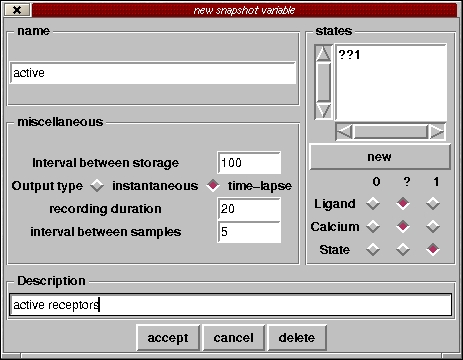
\includegraphics{snaps.jpg}}} A window \emph{Snapshot
  variable [NAME]} pops-up, allowing to configure the snapshot-variable
\emph{NAME}. The name of a snapshot variables is limited to
\MAXARRAYVARNAMELENGTH{} characters.

The frame ``Output characteristics'' allows the configuration of the frequency
and the type of data storage. The ``interval between storage'' specifies the
interval between two storages of the states of the array. Tthe states are
defined in the rightmost frame ``States''. Up to \MAXNUMARRAYSNAPSSTATES{}
states can be represented by each snapshot variable.  If the ``output type'' is
``instantaneous'', the current states of the array is stored. If the ``output
type'' is ``time-lapse'', an average of the states will be stored. The states
will be averaged according the value of ``recording duration'' (which has to be
lower than the ``interval between storage''). The number of averaged snapshot is
deciphered by the value ``interval between samples''(if it is equal to
``recording duration'', only one snapshot is recorded, rendered the output
equivalent to an instantaneous one).

Clicking the three lowest buttons of the \emph{Array [SYMBOL]} window will close it,
either recording the changes, cancelling them or totally removing the array.

\subsection{Creating reactions}\label{reactions}
The reactions are the ``standard'' way for the molecules to interact in the
simulation.  You can select an existing reaction with the browsing list, or
create a new one by clicking on the nearby ``new'' button.

\parpic{\scalebox{0.4}{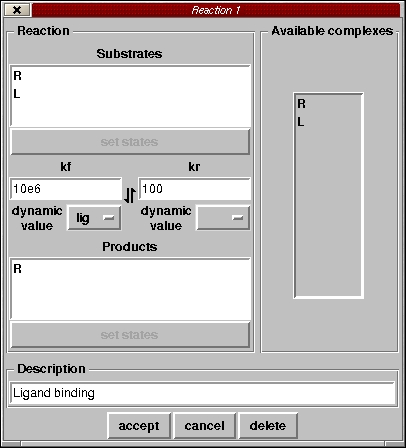
\includegraphics{reaction.jpg}}} A \emph{Reaction X} window
pops-up, allowing the configuration of the reaction \emph{X}. To add a complex as a
substrate or a product, select it in the list on the right, and drag it either in
the substrate list or the product list.  To remove a complex from either the
substrates or the products, select it from the appropriate list and click while
pressing the <Ctrl> key. Note that a reaction has to contain at least one
non-constant substrate and one non-constant product.

Enter the forward and reverse rate in units of s\textsuperscript{-1} or
M\textsuperscript{-1}$\cdot$s\textsuperscript{-1} (according to the order of the
reaction). If a substrate or a product is a multistate complex, you can further
refined the effect of the reaction on the complex, and the effect of the states
on the rate constants.

\vspace{2.5\baselineskip}

\parpic{\scalebox{0.4}{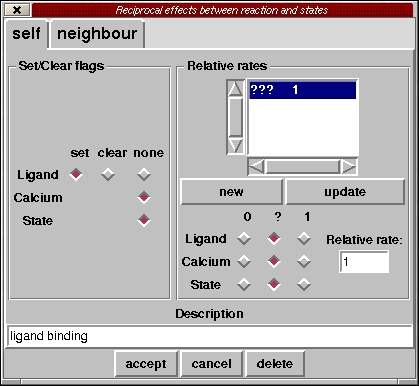
\includegraphics{MSreaction.jpg}}} A click on the button
``set states'' (activated when you select a multistate complex) will pops-up a
new window. Two tabs are present ``self'' and ``neighbour''. The second tab is
activated only when the spatial extensions are used. 

The ``self'' tab permits to configure the classical involvement of a multistate
complex in a reaction.  The left frame permits to set-up the effect of the
reaction on the complex, i.e. to set or clear particular flags. A flag which is
set up by a rapid equilibrium (either multistate or neighbour-sensitive) cannot
be modified here. Change its status first, as explained in the section
\ref{make_multistates}.  The right frame permits to define several states (i.e.
sets of flag values) and their effects on the basal reaction rate.  

\parpic{\scalebox{0.4}{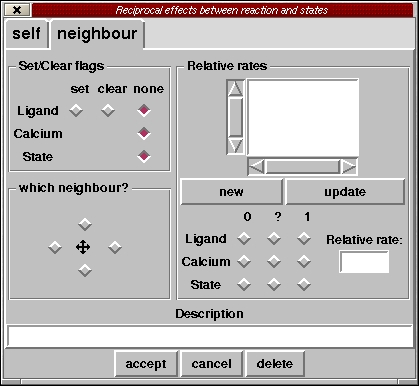
\includegraphics{NSreaction.jpg}}} The ``neighbour'' tab
permits to configure the effect of a neighbour-sensitive complex on the reaction
involving one of its neighbours. The left-top frame permits to set-up the effect
of the reaction on the neighbouring complex, i.e. to set or clear particular
flags. A flag which is set up by a rapid equilibrium (either multistate or
neighbour-sensitive) cannot be modified here. Change its status first, as
explained in the section \ref{make_multistates}.  The right frame permits to
define several states (i.e.  sets of flag values) of the complex and their
effects on the basal rate of the reaction that its neighbour undergoes. Finally
the left-bottom frame allow to choose which neighbour is affected. The number of
possible neighbours depends on the geometry of the lattice containing these
neighbour-sensitive complexes.

Once all the desired values are set, you can commit the changes and quit
(``accept'' button) or quit without recording changes (``cancel'' button).
 
Clicking the three lowest buttons will close the \emph{Reaction} window, either
recording the changes, cancelling them or totally removing the reaction.

\section{Setting-up the dynamic values}

\section{Running a simulation}

Once setup, the simulation can be launched from Tk\stochsim{} by choosing using
``run'' from the ``simulation'' menu, or by typing \mbox{<ctrl-r>}. \emph{Be
  careful, as the configuration is automatically saved before the simulation is
  run}. You can kill this simulation with the item ``stop'' of the ``simulation'' menu.
Note that once \stochsim{} is launched, it is independent of the Tk interface.
When quitting, Tk\stochsim{} \emph{will not kill} \stochsim{}.  When a
simulation has been launched you can load, modify and save other simulations.
You can also visualise the results recorded previously. However you cannot
run another simulation. To do so, launch another instance of the interface.

To quit Tk\stochsim{}, use the menu ``File->Quit'', click the ``quit'' button or
type \mbox{<Ctrl-q>}.

\newpage

\section{Visualisation of the results}\label{display}

You can visualise the result of a simulation, stored in the file
\texttt{VAR.OUT}. To do so, click on the button ``view data'' and a text window
will pops-up. The same result can be achieved with the accelerator <Ctrl-v>.

\scalebox{0.4}{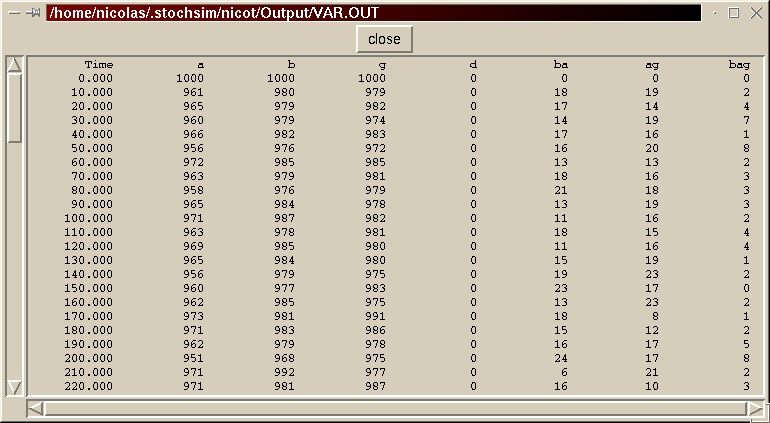
\includegraphics{viewdata.jpg}}

If the button ``show data'' is disabled, either no simulation are loaded, either
the file \texttt{VAR.OUT} does not exist (i.e. the simulation was never run).
Note that you can visualise the results while the simulation is running since
\stochsim{} periodically update the file \texttt{VAR.OUT}.

\parpic{\scalebox{0.4}{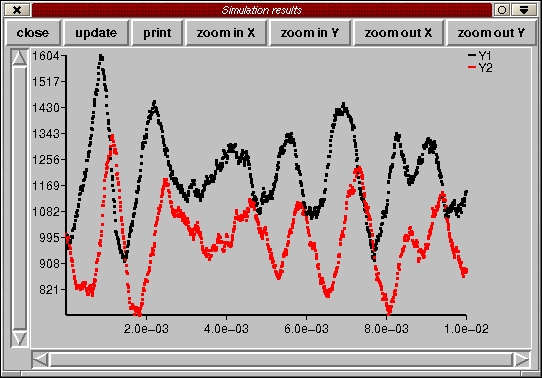
\includegraphics{plot.jpg}}} The results can also be
visualised graphically by clicking the button ``plot''. A graph window will then
pops-up, showing the time course of the variables you chose to display, or of
all the complexes, see section \ref{genconfig}. The same result can be achieved
with the accelerator <Ctrl-p>. The graphs will not automatically refresh.
However you can update them by clicking on the relevant button. The parameters
of the plot can be setup by editing the file \texttt{stochsimrc} directly or via
the menu ``Options>>Preferences''. After choosing a different background color
of plot size, you have to quit and relaunch the plotting window. However the
curves' colors and the type of plot is refreshed with each update. You can
zoom-in and zoom-out the graph, independently for both axis. Choose the
invariant point of the homothetic scaling with <Ctrl-Button1>. You can record
snapshots of the graph at any time, by saving it in a postscript file.

You can monitor the progress of the simulation with a progress bar
launched by the button ``monitor''. The progress bar will refresh itself
automatically. However this consumes memory and cpu time. Therefore it is better
to launch it periodically to probe the simulation progress but to kill it
otherwise.

%%% Local Variables: 
%%% mode: latex
%%% TeX-master: "stochsim_manual"
%%% End: 


\chapter{References}
\begin{itemize}
\item Bray, D., Levin, M. D. \& Morton-Firth, C. J. (1998).  Receptor
clustering as a cellular mechanism to control sensitivity. Nature 393,
85-88.

\item Duke, T. A. J. \& Bray, D.  (1999).  Heightened sensitivity of a
lattice of membrane receptors.  Proc. Natl. Acad. Sci. USA 96,
10104-10108.

\item Gillespie, D. T. (1976). A general method for numerically
simulating the stochastic time evolution of coupled chemical
reactions. J. Comput. Phys. 22, 403-434.

\item Gillespie, D. T. (1977). Exact stochastic simulation of coupled
chemical reactions. J. Phys. Chem. 81, 2340-2361.

\item McAdams, H. H. \& Arkin, A. (1997). Stochastic mechanisms in
gene expression. Proc. Natl. Acad. Sci .USA 94, 814-819.

\item Morton-Firth, C. J. (1998). Stochastic simulation of cell
signalling pathways. Ph.D. Thesis, University of Cambridge.

\item Morton-Firth, C. J. \& Bray, D. (1998). Predicting temporal
fluctuations in an intracellular signalling pathway. J. Theor. Biol.
192, 117-128.

\item Morton-Firth, C. J., Shimizu, T. S. \& Bray, D. (1999). A
free-energy-based stochastic simulation of the Tar receptor complex.
J. Mol. Biol.286, 1059-1074.

\item Shimizu, T.~S., Le~Nov\`{e}re, N., Levin, M.~D., Beavil, A.~J.,
  Sutton, B.~J., and Bray, D. (2000).  Molecular model of a lattice of
  signalling proteins involved in bacterial chemotaxis. Nat. Cell
  Biol. 2, 792--796.

\end{itemize}


\appendix
\chapter[Comparison with the Gillespie algorithm]{\stochsim{}: general description and comparison with the Gillespie algorithm}

The computer program \stochsim{} was written by Carl Firth as part of his
PhD work at the University of Cambridge (Morton-Firth, 1998). It was
developed as part of a study of bacterial chemotaxis as a more
realistic way to represent the stochastic features of this signalling
pathway and also as a means to handle the large numbers of individual
reactions encountered (Morton-Firth \& Bray, 1998; Morton-Firth et
al., 1999). The program provides a general purpose biochemical
simulator in which individual molecules or molecular complexes are
represented as individual software objects. Reactions between
molecules occur stochastically, according to probabilities derived
from known rate constants.  An important feature of the program is its
ability to represent multiple post-translational modifications and
conformational states of protein molecules.

\stochsim{} consists of a platform-independent core simulation engine 
encapsulating the algorithm described above and separate graphical user 
interfaces.   

\section{Description of the algorithm}

Each molecule or molecular species is represented as a separate software object
in \stochsim{}, and the simulation also includes dummy molecules, or 
``pseudo-molecule'' used in the simulation of unimolecular reactions. Time is 
quantised into a series of discrete, independent time-slices, the size of 
which is determined by the most rapid reaction in the system. In each 
time-slice, one molecule (not a pseudo-molecule) is selected at random. Then, 
another object, in this case either a molecule or a pseudo-molecule, is 
selected at random. If two molecules are selected, any reaction that occurs 
will be bimolecular, whereas if one molecule and a pseudo-molecule are 
selected, it will be unimolecular. Another random number is then generated and 
used to see if a reaction occurs; the probability of a reaction is retrieved 
from a look-up table and if the probability exceeds the random number, the 
particles do not react. On the other hand, if the probability is less than the 
random number, the particles react, and the system is updated accordingly. The 
next time-slice then begins with another pair of molecules being selected. 

Whenever a molecule in the system can exist in more than one state then the 
program encodes it as a ``multistate molecule'' with a series of binary flags. 
Each flag represents a state or property of the molecule, such as a 
conformational state; ligand binding; phosphorylation, methylation, or other 
covalent modification. The flags specify the instantaneous state of the 
molecule and may modify the reactions it can perform. For instance, a 
multistate molecule may participate in a reaction at an increased rate as a
result of phosphorylation, or fail to react because it is in an inactive 
conformation. The flags themselves can be modified in each time step as a 
result of a reaction, or they can be instantaneously equilibrated according to 
a fixed probability. The latter tactic is used with processes such as ligand 
binding or conformational change that occur several orders of magnitude faster 
than other chemical reactions in the system. 

If, in a particular time step, \stochsim{} selects one or more multistate 
molecules, then it proceeds in the following manner. First any 
rapidly-equilibrated ``fast flags'' on the molecule are assigned to be on or 
off according to a weighted probability. A protein conformation flag, for 
example, can be set to be active or inactive, according to which other flags 
of the molecules are currently on. A ligand binding flag can, if desired, be 
set in a similar fashion, based on the concentration of ligand and the Kd. 

Once the fast flags have been set, then the program inspects the reactions 
available to species A and B. The chemical change associated with each type of 
reaction (binding, phosphotransfer, methylation, etc.) is represented in the 
program together with a "base values" of the reaction rate constants. The 
particular instantiation of the reaction, determined by the current state of 
the flags on A and B, is accessed from an array of values calculated at the 
beginning of the program, when the reaction system is being initialised. 
Values in the array modify the reaction probability according to the particular
set of binary flags. In this manner, the \stochsim{} calculates a set of 
probabilities, corresponding to the reactions available to the particular 
states of molecules A and B, and then uses a random number to select which 
reaction (if any) will be executed in the next step. The reaction will be 
performed, if appropriate, and the relevant slow flag flipped. 

Although it sounds complicated, the above sequence of events within an 
individual iteration takes place very quickly and even a relatively slow 
computer can carry out hundreds of thousands of iterations every second. 
Moreover, the strategy has the advantage of being intuitively simple and close 
to physical reality. For example, it is easy, if required, to label selected
molecules and to follow their changes with time. Lastly, the speed of the 
program depends not on the number of reactions but on the numbers of molecular 
species in the simulation (with a time of execution proportional to N squared).
  
\section{Comparison with the Gillespie algorithm}

The stochastic simulation of biochemical reactions was pioneered by
Gillespie, who developed an elegant and efficient algorithm for this
purpose (Gillespie, 1976; Gillespie, 1977). Gillespie showed in
rigorous fashion, that his algorithm gives the same result, on
average, as conventional kinetic treatments. In ensuing years, the
algorithm has been widely used to analyse biochemical kinetics and,
most recently, to simulate the stochastic events in lambda lysogeny
(McAdams \& Arkin, 1997). In view of its evident success, the question
therefore arises: Why in our work we did not use the Gillespie
algorithm but chose to develop our own formulation?

The Gillespie algorithm makes time steps of variable length, based on
the rate constants and population size of each chemical species. The
probability of one reaction occurring relative to another is obtained
by multiplying the rate constant of each reaction with the numbers of
its substrate molecules. A random number is then used to choose which
reaction will occur, based on relative probabilities, and another
random number determines how long the step will last. The chemical
populations are altered according to the stoichiometry of the reaction
and the process is repeated. Perhaps because the algorithm was
developed at a time when computers were several thousand times slower
than they are today, it makes extremely efficient use of CPU time. At
each iteration it selects the reaction most likely to occur and
chooses a time step that optimises that reaction, so that the
simulation proceeds extremely efficiently.

However, the efficiency of the Gillespie algorithm comes at a cost.
The elegant algorithm that selects which reaction to perform, and what
time interval to take, cannot represent individual molecular events in
the reaction. With regard to the reactions of a typical cell
signalling pathway, for example, it cannot associate physical
quantities with each molecule, nor trace the fate of particular
molecules over a period of time. This means that it is not possible to
extend this algorithm to a more thermodynamically realistic model in
which energies and conformational states are associated with each
molecule.  Similarly, without the ability to associate positional and
velocity information with each particle, the algorithm cannot be
adapted to simulate diffusion, localisation or spatial heterogeneity.

A second deficiency of the Gillespie algorithm (from a cell biological
standpoint) is that it cannot easily handle the reactions of
multi-state molecules. Protein molecules are very frequently modified
in the cell so as to alter their catalytic activity, binding affinity
and so on. Cell signalling pathways, for example, carry information in
the form of chemical changes such as phosphorylation or methylation,
or as conformational state. A multi-protein complex may contain
upwards of twenty sites, each of which can often be modified
independently and each of which can, in principle, influence how the
complex will participate in chemical reactions. With twenty sites, a
complex can exist in a total of 2\textsuperscript{20}, or one million,
unique states, each of which could react in a slightly different way.
If our multi-protein complex interacts with only ten other chemical
species, a detailed model may contain as many as ten million distinct
chemical reactions,  a combinatorial explosion.  Any program in which
the time taken increases in proportion to the number of reactions, as
in a conventional, deterministic model, or in the Gillespie method,
will come to a halt under these conditions.

To summarise, \stochsim{} is likely to be slower than the Gillespie
algorithm in calculating the eventual outcome of a small set of simple
biochemical reactions, especially when the numbers of molecules is
large. However, if the system contains molecules that can exist in
multiple states, then \stochsim{} will not only be faster but also
closer to physical reality. It is easy, if required, to label selected
molecules in this program and to follow their changes with time,
including changes to their detailed post-translational modification
and conformational state. Although the program does not, in its
present form, incorporate spatial information regarding the positions
of molecules, we have found that such modification can be made in a
straightforward manner.
%%% Local Variables: 
%%% mode: latex
%%% TeX-master: "stochsim_manual"
%%% End: 

  
\end{document}
